
% !TeX root = main.tex

%%%%%%%%%%%%%%%%%%%%%%%%%%%%%%%%%%%%%%%%%%%%%%%%%%
%%%%%%%%%%%%%%%%%%%%% preamble %%%%%%%%%%%%%%%%%%%
%%%%%%%%%%%%%%%%%%%%%%%%%%%%%%%%%%%%%%%%%%%%%%%%%%
\documentclass[11pt,openany,a4paper]{book}
\usepackage[mono=false]{libertine} % new linux font, ignore mono
\usepackage{luatex85}
%\renewcommand{\baselinestretch}{1.05}
\usepackage{amsmath,amsthm,amssymb,mathrsfs,amsfonts,dsfont,bbm}
\usepackage{epsfig,graphicx}
\usepackage{tabularx}
\usepackage{blkarray}
\usepackage{slashed}
\usepackage{xcolor}
\usepackage{csquotes}
\usepackage{listings,soul}
\usepackage{caption}
\usepackage{subcaption}
\usepackage{ragged2e}% \usepackage{fullpage}
\usepackage{lipsum} % provides dummy text for testing
\usepackage[toc,title,titletoc,header]{appendix}
\usepackage{etoc} 
\etocsetnexttocdepth{subsection}
\usepackage{multicol} % two-col ToC
\usepackage{bm}
\usepackage{imakeidx} % before hyperref
\usepackage{hyperref}
\usepackage[brazilian]{babel}
% link colors settings
\definecolor{magentao}{rgb}{.75, 0, .25 } 
\hypersetup{
	colorlinks=true, linkcolor = black, urlcolor=magentao, citecolor=magentao
 %[rgb]{0.0, 0.14, 0.6}
}
\usepackage[capitalise]{cleveref}
\usepackage{enumitem}
\usepackage{mathtools}
\usepackage{physics}
\usepackage[linesnumbered,ruled,vlined,algosection]{algorithm2e}
\SetCommentSty{textsf}
\usepackage{epigraph}
\epigraphwidth=1.0\linewidth
\epigraphrule=0pt

% adjust margin
\usepackage[margin=2.3cm]{geometry}
\headheight13.6pt

%%%%%%%%%%%%%%%% thmtools %%%%%%%%%%%%%%%%%%%%%
\usepackage{thmtools}
\declaretheorem[numberwithin=chapter]{theorem}
\declaretheorem[numberwithin=chapter]{axiom}
\declaretheorem[numberwithin=chapter]{lemma}
%\declaretheorem[numberwithin=chapter]{proposição}
\declaretheorem[numberwithin=chapter]{claim}
\declaretheorem[numberwithin=chapter]{conjecture}
\declaretheorem[sibling=theorem]{corollary}
\declaretheorem[style=definition]{definição}
\declaretheorem[numberwithin=chapter, style=definition]{problem}
\declaretheorem[numberwithin=chapter, style=definition]{example}
\declaretheorem[numberwithin=chapter, style=definition]{exercise}
\declaretheorem[numberwithin=chapter, style=definition]{observation}
\declaretheorem[numberwithin=chapter, style=definition]{fact}
\declaretheorem[numberwithin=chapter, style=definition]{construction}
\declaretheorem[numberwithin=chapter, style=definition]{remark}
\declaretheorem[numberwithin=chapter, style=remark]{question}
%%%%%%%%%%%%%%%% thmtools %%%%%%%%%%%%%%%%%%%%%
\usepackage{changepage}
\newenvironment{solution}
    {\renewcommand\qedsymbol{$\square$}\color{blue}\begin{adjustwidth}{0em}{2em}\begin{proof}[\textit Solution.~]}
    {\end{proof}\end{adjustwidth}}

%%%%%%%%%%%%%%%% index %%%%%%%%%%%%%%%%%%%%%
\begin{filecontents}{index.ist}
% https://tex.stackexchange.com/questions/65247/index-with-an-initial-letter-of-the-group
headings_flag 1
heading_prefix "{\\centering\\large \\textbf{"
heading_suffix "}}\\nopagebreak\n"
delim_0 "\\nobreak\\dotfill"
\end{filecontents}
\newcommand{\myindex}[1]{\index{#1} \emph{#1}}
\makeindex[columns=3, intoc, title=Alphabetical Index, options= -s index.ist]
%%%%%%%%%%%%%%%% index %%%%%%%%%%%%%%%%%%%%%

%%%%%%%%%%%%%%%% ToC %%%%%%%%%%%%%%%%%%%%%
% Link Chapter title to ToC: https://tex.stackexchange.com/questions/32495/linking-the-section-text-to-the-toc
\usepackage[explicit]{titlesec}
\titleformat{\chapter}[display]
  {\normalfont\huge\bfseries}{\chaptertitlename\ {\thechapter}}{20pt}{\hyperlink{chap-\thechapter}{\huge#1}
\addtocontents{toc}{\protect\hypertarget{chap-\thechapter}{}}}
\titleformat{name=\chapter,numberless}
  {\normalfont\huge\bfseries}{}{-20pt}{\huge#1}


%%%%%%%%%%%%%%%%%%% fancyhdr %%%%%%%%%%%%%%%%%
\usepackage{fancyhdr}
\pagestyle{fancy} % enable fancy page style
\renewcommand{\headrulewidth}{0.0pt} % comment if you want the rule
\fancyhf{} % clear header and footer
\fancyhead[lo,le]{\leftmark}
\fancyhead[re,ro]{\rightmark}
\fancyfoot[CE,CO]{\hyperref[toc-contents]{\thepage}}

% https://tex.stackexchange.com/questions/550520/making-each-page-number-link-back-to-beginning-of-chapter-or-section
\makeatletter
\def\chaptermark#1{\markboth{\protect\hyper@linkstart{link}{\@currentHref}{Capítulo \thechapter ~ #1}\protect\hyper@linkend}{}}
\def\sectionmark#1{\markright{\protect\hyper@linkstart{link}{\@currentHref}{\thesection ~ #1}\protect\hyper@linkend}}
\makeatother
%%%%%%%%%%%%%%%%%%% fancyhdr %%%%%%%%%%%%%%%%%


%%%%%%%%%%%%%%%%%%% biblatex %%%%%%%%%%%%%%%%%
\usepackage[doi=false,url=false,isbn=false,style=authoryear,backend=biber,backref=true]{biblatex}
\addbibresource{bib.bib}

\newbibmacro{string+doiurlisbn}[1]{%
  \iffieldundef{doi}{%
    \iffieldundef{url}{%
      \iffieldundef{isbn}{%
        \iffieldundef{issn}{%
          #1%
        }{%
          \href{http://books.google.com/books?vid=ISSN\thefield{issn}}{#1}%
        }%
      }{%
        \href{http://books.google.com/books?vid=ISBN\thefield{isbn}}{#1}%
      }%
    }{%
      \href{\thefield{url}}{#1}%
    }%
  }{%
    \href{http://dx.doi.org/\thefield{doi}}{#1}%
  }%
}

% https://tex.stackexchange.com/questions/94089/remove-quotes-from-inbook-reference-title-with-biblatex
\DeclareFieldFormat[article,incollection,inproceedings,book,misc]{title}{\usebibmacro{string+doiurlisbn}{\mkbibemph{#1}}}
% https://tex.stackexchange.com/questions/454672/biblatex-journal-name-non-italic
\DeclareFieldFormat{journaltitle}{#1\isdot}
\DeclareFieldFormat{booktitle}{#1\isdot}
% https://tex.stackexchange.com/questions/10682/suppress-in-biblatex
\renewbibmacro{in:}{}
% add video field: https://tex.stackexchange.com/questions/111846/biblatex-2-custom-fields-only-one-is-working
\DeclareSourcemap{
    \maps[datatype=bibtex]{
      \map{
        \step[fieldsource=video]
        \step[fieldset=usera,origfieldval]
    }
  }
}
\DeclareFieldFormat{usera}{\href{#1}{\textsc{Online video}}}
\AtEveryBibitem{
    \csappto{blx@bbx@\thefield{entrytype}}{% put at end of entry
        \iffieldundef{usera}{}{\space \printfield{usera}}
    }
}

\input{auxiliary/macros.tex}

\newtheorem{prop}{Proposição}
\newtheorem{defin}{Definição}
\newtheorem{teo}{Teorema}

%%%%%%%%%%%%%%%%%%%%%%%%%%%%%%%%%%%%%%%%%%%%%%%%%%
%%%%%%%%%%%%%%%% begin of document %%%%%%%%%%%%%%%
%%%%%%%%%%%%%%%%%%%%%%%%%%%%%%%%%%%%%%%%%%%%%%%%%%

\begin{document}
\frontmatter
\title{\bf \huge Notas de Aula: \\
        Desenho de Mercados}
\author{Pedro Henrique Chaves Maia}
\date{Atualizado em \today \\ (\href{https://gvmail-my.sharepoint.com/:b:/g/personal/b30993_fgv_edu_br/EdV2A8MLs21Fto6W-hhC1M0Be7SeWx1q7JrGajWqVmkwbw?e=iTQJT1}{{\sc Versão mais atualizada}})}
\maketitle
\setcounter{tocdepth}{2}

\begin{multicols*}{2}
    \tableofcontents
    \label{toc-contents}
\end{multicols*}

%%%%%%%%%%%%%% minitoc $%%%%%%%%%%%
\etocsettocstyle{\vskip-2\baselineskip\noindent\rule{\linewidth}{0.5pt}\vskip0.3\baselineskip}%
    {\noindent\rule{\linewidth}{0.5pt}\vskip0.5\baselineskip}
    
%%%%%%%%%%%%%%% Content %%%%%%%%%%%%%%%
\mainmatter % separates the number of toc and mainmatter
\chapter*{Prefácio}
\addcontentsline{toc}{chapter}{Prefácio}


Este manual é um compêndio das notas de aula do curso "Desenhos de Mercados", ministrado pelo Prof. Fulvio Fontini. Todos os materiais aqui expostos podem ser recuperados - e melhor representados - em \textcite{cretì_fontini_2019}, material original no qual o curso se baseia.

\section*{Contato}
Eu construí esse material na melhor das intenções e cuidado, mas, naturalmente, erros podem ser encontrados. Por favor, caso encontre algum erro ou tenha comentários a fazer, entre em contato comigo por \href{mailto:maia.pedro@fgv.edu.br}{maia.pedro@fgv.edu.br}.

\section*{Copyright e Licença}

\begin{itemize}
    \item \href{https://github.com/Jue-Xu/Latex-Template-for-Scientific-Style-Book}{GitHub Repo do template}
    \item \href{https://www.overleaf.com/latex/templates/latex-template-for-scientific-style-book/ntprxjksmqxx}{Overleaf template}
\end{itemize}




\part{Matemática}
\chapter{Condições de Karush-Kuhn-Tucker (KKT) \label{kkt}}

\localtableofcontents % local TOC <<<<<<<<<<<<<<<<<<<<<<<<<<<<<<<<<,


Na otimização matemática, as condições de Karush-Kuhn-Tucker (KKT), também conhecidas como condições de Kuhn-Tucker, são testes de primeira derivada (às vezes chamados de condições necessárias de primeira ordem) para que uma solução em programação não linear seja ótima, desde que alguns condições de regularidade são satisfeitas. Permitindo restrições de desigualdade, a abordagem KKT para programação não linear generaliza o método dos multiplicadores de Lagrange, limitado à restrições de igualdade. Semelhante à abordagem de Lagrange, o problema de maximização (minimização) restrita é reescrito como uma função de Lagrange cujo ponto ótimo é um ponto de sela.

O argumento aqui construído é fortemente baseado nas notas de aula de \textcite{tibshirani_convex_2015}.

\section{Problema Dual}
\subsection{Construção}
Suponha o problema de programação não linear:
\begin{align*}
    \min_{x \in \mathbb{R}^n}&\quad f(x)\\
    \text{s.a.}&\quad h_i(x) \le b_i, i = 1,..m\\
    &\quad l_j(x)  = k_j, j = 1,...r 
\end{align*}
onde as funções acima não precisam ser, necessariamente, convexas. Podemos escrever o Lagrangiano:
\begin{align*}
    \mathcal{L}(x,\lambda,\mu)  = f(x) + \sum_i\lambda_i(h_i(x)-b_i) + \sum_j\mu_j(l_j(x)-k_j)
\end{align*}
Restrinja $\lambda_i$ a ser não-negativo. Uma propriedade do Lagrangiano é:
\begin{align*}
    f(x) \ge \mathcal{L}(x,\lambda,\mu)
\end{align*}
Onde $x$ é factível. Ou seja, $\mathcal{L}$ é um limite inferior de $f(x)$ sobre o conjunto factível $C$. Minimizando dos dois lados temos:
\begin{align*}
    f^* \ge \min_{x \in C}\mathcal{L}(x,\lambda,\mu) \ge \min_{x \in \mathbb{R}^n}\mathcal{L}(x,\lambda,\mu) \equiv g(\lambda,\mu)
\end{align*}
onde $g(\lambda,\mu)$ é chamada de \textit{função dual}, que informa um limite inferior do valor ótimo $f^*$ para o problema primal. Para obter o melhor limite inferior, $g$ é maximizando sobre $\lambda,\mu$, implicando o problema dual
\begin{align*}
    \max_{\lambda \in \mathbb{R}^m, \mu \in \mathbb{R}^r}&\quad g(\lambda,\mu)\\
    \text{s.a.}&\quad \lambda\geq0
\end{align*}

\subsection{Propriedades}
\paragraph{Dualidade Fraca} Por construção, $f^* \ge g^*$  é sempre verdade (mesmo se o problema primal não for convexo).
\paragraph{Convexidade do Problema Dual} O problema dual é sempre convexo i.e. $g$ é sempre côncava (novamente, mesmo se o problema primal não for convexo). 
\paragraph{Condição de Slater} Para problemas primals convexos, se existe um $x$ tal que $h_i(x)<b_i$ e $l_j(x)=k_j$ para todo $i,j$, então temos \textbf{dualidade forte} i.e. $f^*=g^*$.

\subsection{Distância de Dualidade (Duality Gap)}
Dado um primal factível $x$ e dual factível $\lambda, \mu$, a quantidade
\[ f(x) - g(\lambda,\mu)\]
é chamada de distância de dualidade entre $x$ e $\lambda, \mu$. Note que
\[  f(x) - f(x^*) \ge  f(x) - g(\lambda, \mu)\]
por construção. Logo, se a distância de dualidade for zero, então $x$ é ótimo primal (e, da mesma forma, $\lambda, \mu$ são ótimos duais). 
\medskip

\noindent\fbox{%
    \parbox{\textwidth}{%
        Note que, do ponto de vista algorítmico, fornece um critério de parada: 
        \medskip
        
        se $f(x) - g(\lambda, \mu) \le \varepsilon$, então garantimos que $f(x) - f^* \le \varepsilon$. Muito útil, especialmente em conjunto com métodos iterativos!
    }%
}
\section{Condições Karush-Kuhn-Tucker (KKT)} 
Seja um problema primal tal qual descrito na seção anterior. Temos que as condições KKT são:
\begin{enumerate}
    \item \textbf{Estacionariedade}: $\partial\mathcal{L}(x)\in0$ ou, mais comumente representado, $\frac{\partial\mathcal{L}}{\partial x_n}=0$ para todo $n=1,...,N$. Indica que $x$ minimiza o Lagrangiano sobre todo $x$.
    \item \textbf{Frouxidão Complementar}: $\lambda_i\cdot h_i(x) = 0$ para todo $i$. Se $h_i(x)$ for estritamente menor que zero, então $\lambda_i = 0$. Se $h_i(x)$ igual a zero, então $\lambda_i$ pode assumir qualquer valor.
    \item \textbf{Factibilidade Primal}: $h_i(x) \le b_i$, $l_j(x) = k_j$ para todo $i, j$.
    \item \textbf{Factibilidade Dual}: $\lambda_i\geq0$ para todo $i$.
\end{enumerate}
Seguem abaixo duas importantes proposições:
\paragraph{Proposição 1} (Necessidade) Se $x^*$ e $\lambda^*,\mu^*$ são soluções primais e duais, com distância de dualidade zero, então $x^*$, $\lambda^*,\mu^*$ satisfazem as condições KKT.

\paragraph{Proposição 2} (Suficiência) Se $x^*$ e $\lambda^*,\mu^*$ satisfazem as condições KKT, então $x^*$, $\lambda^*,\mu^*$ são soluções primais e duais.

Ou seja, para problemas convexos (Condição de Slater valendo), temos que $x^*$, $\lambda^*,\mu^*$ são soluções primais e duais se, e somente se, atendem às condições KKT.

\section{Exemplos}
\begin{enumerate}
    \item[1)] Resolva o seguinte problema de otimização não-linear:
        \begin{align*}
            \max_{x,y\in\mathbb{R}}&\quad f(x,y)=xy \\
            \text{s.a.}&\quad x+y^2\le 2\\
            &\quad x,y\geq0
        \end{align*}
        \textbf{Resposta:}
        \textcolor{magentao}{
        Observe que a região factível é limitada, então um máximo global deve existir: uma função contínua em um conjunto fechado e limitado possui, sempre, um máximo global (Teorema do Valor Extremo). Mais ainda, repare que $f(x,y)$ é uma função convexa, logo as condições KKT são suficientes para encontrar os máximos globais. Vamos reescrever o problema em termos que já estamos acostumados:
        \begin{align*}
            \min_{x,y\in\mathbb{R}}&\quad -xy \\
            \text{s.a.}&\quad x+y^2\le 2\\
            &\quad -x\le0\\
            &\quad -y\le0
        \end{align*}
        Implicando o Lagrangiano
        \begin{align*}
            \mathcal{L}(x,y,\lambda_1,\lambda_2,\lambda_3) = -xy + \lambda_1 (x+y^2-2) + \lambda_2(-x-0) + \lambda_3(-y-0)
        \end{align*}
        Vamos enunciar as condições KKT:
        \begin{enumerate}
            \item \textbf{Estacionariedade}:
            \begin{align*}
                \frac{\partial\mathcal{L}}{\partial x} &= -y+\lambda_1-\lambda_2 = 0\\
                \frac{\partial\mathcal{L}}{\partial y} &= -x +2\lambda_1y - \lambda_3 = 0
            \end{align*}
            \item \textbf{Frouxidão Complementar}: 
            \begin{align*}
                 \lambda_1 (x+y^2-2) &= 0 \\
                 -\lambda_2x &= 0 \\
                 -\lambda_2y &= 0 
            \end{align*}
            \item \textbf{Factibilidade Primal}
            \begin{align*}
                x+y^2 &\le 2\\
                -x&\le0\\
                -y&\leq0
            \end{align*}
            \item \textbf{Factibilidade Dual:}
            \begin{align*}
                \lambda_1,\lambda_2,\lambda_3\ge0
            \end{align*}
        \end{enumerate}
        Seja $n$ o número de restrições. Pela natureza do sistema acima, sempre teremos $2^n$ possíveis casos a considerar (equivalente a 8 casos, nesse exemplo). Entretanto, refletindo sobre o problema podemos reduzir esse número substancialmente:
        \begin{enumerate}
            \item[\textbf{Caso 1}] \underline{Suponha que $\lambda_1 = 0$}. Então a primeira condição KKT implica $y + \lambda_2 = 0$ e a segunda $x + \lambda_3 = 0$. Como cada termo é não negativo, a única maneira de isso acontecer é se $x = y = \lambda_2 = \lambda_3 = 0$. De fato, as condições KKT são satisfeitas quando $x = y = \lambda_1 = \lambda_2 = \lambda_3 = 0$ (embora claramente este não seja um máximo local, já que $f(0, 0) = 0$ enquanto existem $x,y$ no interior da região factível t.q. $f(x, y) > 0$ - (1,1), por exemplo).
            \item[\textbf{Caso 2}] \underline{Suponha $\lambda_1 \neq 0$ i.e. $x + y^2 = 2$}. Para que isso seja possível, note que deve valer $x = 2 - y^2>0$ ou $y>0$.
            \begin{enumerate}
                \item[\textbf{Caso 2a)}] \underline{Suponha que $x > 0$}. Então $\lambda_2 = 0$. A primeira condição KKT implica $\lambda_1 = y$. A segunda condição KKT implica $x - 2y\lambda_1 + \lambda_3 = 2 - 3y^2 + \lambda_3 = 0$, então $3y^2 = 2 + \lambda_3 > 0$, e $\lambda_3 = 0$. Portanto, $y = \sqrt{2/3}$ e $x = 2 - 2/3 = 4/3$. Repare que, por construção, todas as condições KKT são satisfeitas.
                \item[\textbf{Caso 2b)}] \underline{Suponha que $x = 0$}, ou seja, $y = \sqrt{2}$. Como $y > 0$ temos $\lambda_3 = 0$. A partir da segunda condição KKT, devemos ter $\lambda_1 = 0$, mas isso nos leva de volta ao Caso 1. Concluímos que há apenas dois candidatos a um máximo local: $(0, 0)$ e$(4/3,\sqrt{2/3})$. O máximo global é em $(4/3,\sqrt{2/3})$.
            \end{enumerate}
        \end{enumerate}
        }
    \item[2)] Resolva o seguinte problema de otimização não-linear:
    \begin{align*}
        \max_{x_1,x_2\in\mathbb{R}}&\quad f(x_1,x_2)=3.6x_1 -0.4x_1^2+1.6x_2-0.2x_2^2\\
        \text{s.a.}&\quad 2x_1 + x_2\le10\\
        &\quad x_1,x_2\ge0
    \end{align*}
    \textbf{Resposta}:
    \textcolor{magentao}{
    Tal qual no item anterior, repare que a função acima é contínua sendo maximizada num conjunto compacto - portanto há máximo global. Mais ainda, é uma função convexa, logo KKT é condição necessária e suficiente. Começamos reescrevendo o problema:
    \begin{align*}
            \min_{x,y\in\mathbb{R}}&\quad-3.6x_1 +0.4x_1^2-1.6x_2+0.2x_2^2\\
            \text{s.a.}&\quad 2x_1 + x_2\le10\\
            &\quad x_1,x_2\ge0
    \end{align*}
    Repare que no último exercício as condições de factibilidade primal de positividade dos argumentos de $f(\cdot,\cdot)$ poderiam ser ignoradas (e com isso $\lambda_2$ e $\lambda_3$). Isso é geralmente verdade para problemas convexos e, portanto, ignorarei os multiplicadores de Lagrange deles nesse item (recomendo que sempre façam isso). O Lagrangiano será, portanto:
    \begin{align*}
        \mathcal{L}(x_1,x_2,\lambda) =  -3.6x_1 +0.4x_1^2-1.6x_2+0.2x_2^2 + \lambda(2x_1 + x_2-10)
    \end{align*}
    Implicando as seguintes restrições
    \begin{align*}
        \begin{aligned}
        -3.6+0.8x_1+2\lambda = 0\\
        -1.6 +0.4x_2+\lambda=0 
        \end{aligned} &&
        \left. \begin{aligned}
           \text{ }\\
           \text{ }
        \end{aligned}  \right\rbrace && \qquad \text{\textbf{Estacionariedade}}\\
        \begin{aligned}
            \lambda(2x_1 + x_2-10)=0
        \end{aligned} &&
         \left. \begin{aligned}
           \text{ }
        \end{aligned}  \right\rbrace && \qquad \text{\textbf{Frouxidão Complementar}}\\
        \begin{aligned}
            \lambda\ge0
        \end{aligned} &&
        \left. \begin{aligned}
           \text{ }
        \end{aligned}  \right\rbrace && \qquad \text{\textbf{Factibilidade Dual}}\\
        \begin{aligned}
            2x_1 + x_2\le10\\
            x_1,x_2\ge0
        \end{aligned} && 
        \left. \begin{aligned}
           \text{ }\\
           \text{ }
        \end{aligned}  \right\rbrace && \qquad \text{\textbf{Factibilidade Primal}}\\
    \end{align*}
    Temos, portanto, apenas dois casos:
    \begin{enumerate}
        \item[\textbf{Caso 1)}] \underline{Seja $\lambda=0$}. Das condições de estacionariedade temos que $x_1=4.5$ e $x_2 = 4$. Repare que, para esses valores, a primeira condição de factibilidade primal não valerá. Portanto, essa resposta não pode ser solução para o problema.
        \item[\textbf{Caso 2}] \underline{Seja $\lambda\neq0$ i.e. $2x_1 + x_2=10$}. Como só temos 2 casos e sabemos, pelo Teorema do Valor Extremo, que existe solução, essa é deve ser a resposta. Das condições de estacionariedade temos $x_1=\frac{3.6-2\lambda}{0.8}$ e $x_2=\frac{1.6-\lambda}{0.4}$. Usando que $2x_1 + x_2=10$ temos que $\lambda=0.4$. Aplicando em $x_1$ e $x_2$ encontramos $(x_1,x_2)=(3.5,3)$. Note que todas as condições KKT são atendidas e, portanto, esse é o máximo do problema primal.
    \end{enumerate}
    }
\end{enumerate}
\section{Interpretação dos Multiplicadores de Lagrange}
Os multiplicadores de Lagrange $\lambda$ são mais que, apenas, mecanismos matemáticos para recuperar os parâmetros desejados. A interpretação exata dessa variável depende do contexto em específico da questão, entretanto, é possível ter alguma informação sobre a intuição dela da derivação matemática do Lagrangiano. Repare que (pensando no problema de otimização no começo da lista):
\begin{align*}
    \frac{\partial\mathcal{L}}{\partial b_i} = \lambda_i
\end{align*}
Ou seja, $\lambda_i$ informa a taxa de crescimento instantânea do Lagrangiano quando relaxamos a restrição $b_i$ em um $\varepsilon$ infinitesimal. Em outras palavras, o multiplicador representa os ganhos líquidos marginais de se relaxar a respectiva restrição. Ou ainda, o multiplicador de Lagrange fornece a taxa de variação da solução para o problema de maximização restrita à medida em que a restrição varia. 

\part{Economia da Eletricidade}
\chapter{Problema Centralizado de Despacho Ótimo}
\localtableofcontents 

Este capítulo é baseado nas notas de aula do curso, ministrado em 10/08/2023, e nas informações do Capítulo 8 de \textcite{cretì_fontini_2019}.

\section{Introdução ao Problema}
Neste capítulo, analisamos o problema de fornecer eletricidade para atender à carga a partir de uma variedade de usinas de energia de maneira ótima. Como é comum em economia, consideramos a eficiência de Pareto como critério de otimização. Não levamos em conta externalidades, bens públicos e questões distribucionais.

Assuma que o sistema possui uma carga (\textit{load}) fixa $\overline{Q}>0$. Assuma um monopolista que detenha um número $I$ de usinas de geração elétrica com diferentes estruturas de custo $c_i(q_i)$. Defina o Bem-Estar Social como $W \equiv u(Q)-\sum_ic_i(Q)$, onde $u(\cdot)$ é a utilidade da sociedade com respeito ao consumo de eletricidade. Assuma, de forma geral e pelo resto do curso, as propriedades usuais para função custo e utilidade i.e. $u'(\cdot)>0, u''(\cdot)\le0,c'(\cdot)>0,c''(\cdot)\ge0,u(0)=0$.

Mais ainda, note que como a carga do sistema é tomada exogenamente i.e. os agentes (consumidores) consomem agregadamente uma quantidade fixa de eletricidade, independente de qualquer outro fator, temos que $W=u(\overline{Q})-\sum_ic_i(Q)$. Mais ainda, nesse contexto o problema do monopolista que minimiza custos é idêntico ao de um planejador central que maximiza o bem-estar. Essa relação é chamada de "problema dual", entretanto, não confunda com o problema dual das condições de KKT (ver Capítulo~\ref{kkt}).
\section{O Problema do Monopolista}
Explicitamente, assuma $I=2$. O problema do monopolista pode ser parcialmente escrito como:
\begin{align*}
    \min_{q_1,q_2\in\mathbb{R}}&\quad c_1(q_1) + c_2(q_2)\\
    \text{s.a.}&\quad 0\le q_1\le q_1^{max}\\
    &\quad 0\le q_2\le q_2^{max}\\
    &\quad 0\le q_1\le q_1^{max}\\
    &\quad q_1+q_2=\overline{Q}
\end{align*}
Podemos, então, escrever o Lagrangiano do problema como:
\begin{align*}
    \mathcal{L}=c_1(q_1) + c_2(q_2) +\mu(q_1+q_2-\overline{Q}) +\lambda_1 (-q_1) +\lambda_2 (-q_2) + \lambda_3(q_1-q_1^{max})+ \lambda_4(q_2-q_2^{max})    
\end{align*}

Como já assumimos que $c_i(\cdot)\ge0$ i.e. as funções custo são (quasi-)convexas, temos que as condições KKT são suficientes para determinar o ótimo do programa não-linear descrito acima. Explicitamente, as condições KKT para este problema são:
\begin{align*}
    \begin{aligned}
        \frac{\partial\mathcal{L}}{\partial q_1} &= c_1'(q_1) + \mu - \lambda_1 + \lambda_3 = 0\\
        \frac{\partial\mathcal{L}}{\partial q_2} &= c_2'(q_2) + \mu - \lambda_2 + \lambda_4 =0 
        \end{aligned} &&
        \left. \begin{aligned}
           \text{ }\\
           \text{ }
        \end{aligned}  \right\rbrace && \qquad \text{\textbf{Estacionariedade}}\\
        \begin{aligned}
            \lambda_1 (-q_1)&=0 \\
            \lambda_2 (-q_2)&=0 \\
            \lambda_3(q_1-q_1^{max})&=0\\
            \lambda_4(q_2-q_2^{max})&=0
        \end{aligned} &&
         \left. \begin{aligned}
           \text{ } \\
           \text{ } \\
           \text{ } \\
           \text{ } 
        \end{aligned}  \right\rbrace && \qquad \text{\textbf{Frouxidão Complementar}}\\
        \begin{aligned}
            \lambda_1,\lambda_2,\lambda_3,\lambda_4\ge0
        \end{aligned} &&
        \left. \begin{aligned}
           \text{ }
        \end{aligned}  \right\rbrace && \qquad \text{\textbf{Factibilidade Dual}}\\
        \begin{aligned}
            0\le q_1&\le q_1^{max}\\
            0\le q_2&\le q_2^{max}\\
            0\le q_1&\le q_1^{max}\\
            q_1+q_2&=\overline{Q}
        \end{aligned} && 
        \left. \begin{aligned}
           \text{ }\\
           \text{ }\\
           \text{ }\\
           \text{ } 
        \end{aligned}  \right\rbrace && \qquad \text{\textbf{Factibilidade Primal}}\\
\end{align*}
Suponha, com \textit{pouca perda de generalidade}, que $c_1'(q_1)<c_2'(q_2)$ para todo $q_1,q_2\in\mathbb{R}$. Note, entretanto, que, da forma como escrito acima, o problema é indefinido, ou seja, precisa de mais restrições. 

\subsection{Caso $q_1^{max},q_2^{max}>\overline{Q}$}
Repare que assumirmos $q_1^{max},q_2^{max}>\overline{Q}$ implica $q_1^*<q_1^{max}$ e $q_2^*<q_2^{max}$ pois, caso contrário, teríamos uma violação da factibilidade primal ($q_1^*+q_2^*>\overline{Q}$). Logo, pela frouxidão complementar, temos que $\lambda_3=\lambda_4=0$. Destarte, podemos reescrever as condições de estacionariedade da seguinte forma:
\begin{align*}
    \begin{cases}
        c_1'(q_1) = -\mu+\lambda_1\\
        c_2'(q_2) = -\mu+\lambda_2
    \end{cases}
\end{align*}
Teremos então que, de $c_1(\cdot)<c_2(\cdot)$:
\begin{align*}
     -\mu+\lambda_1< -\mu+\lambda_2 \Longleftrightarrow \lambda_1<\lambda_2
\end{align*}
Temos, portanto, dois possíveis casos para que a condição acima seja verdade.
\begin{enumerate}
    \item[1)] Suponha que $\lambda_1>0$ t.q. $\lambda_1<\lambda_2$. Ora, então teríamos, por frouxidão complementar, que $q_1^*=q_2^*=0$. Esse resultado claramente não atende factibilidade primária, pois implica $\overline{Q}=0$, e, portanto, não pode ser solução do problema de otimização. 
    \item[2)] Suponha que $\lambda_1=0$, implicando $\lambda_2>0$. Teríamos então, por frouxidão complementar, que $q_1^*>0$ e $q_2^*=0$ t.q. $q_1^*+q_2^*=\overline{Q}$ (por factibilidade primal), implicando por sua vez $q_1^*=\overline{Q}$. Repare que esse resultado atende à todas as condições KKT sendo, portanto, solução do problema de otimização.
\end{enumerate}
Concluímos, então, que a usina mais eficiente (com o menor custo marginal) é aquela que atende toda a carga exógena $\overline{Q}$. Em específico, supondo forma funcional
\[c_i(q_i)=FC_i+c_i'q_i\]
Temos a representação gráfica do problema dada pela Figura~\ref{fig:dispatching_1}.
\begin{figure}
    \centering
    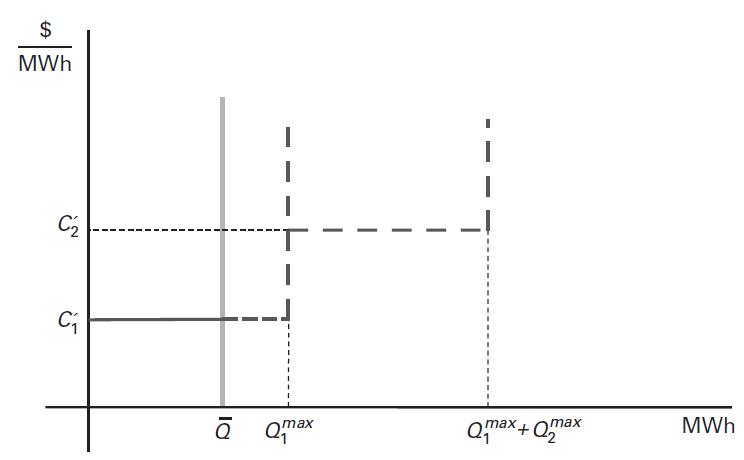
\includegraphics[scale=.4]{figure/dispatching_1.png}
    \caption{Despachamento Ótimo quando $q_1^{max},q_2^{max}>\overline{Q}$}
    \label{fig:dispatching_1}
\end{figure}

\subsection{Caso $q_1^{max},q_2^{max}<\overline{Q}$}
Repare que assumirmos $q_1^{max},q_2^{max}<\overline{Q}$ implica $q_1^*,q_2^*>0$, pois, caso contrário, teríamos uma violação da factibilidade primal ($q_1^*+q_2^*<\overline{Q}$). Logo, pela frouxidão complementar, temos que $\lambda_1=\lambda_2=0$. Destarte, podemos reescrever as condições de estacionariedade da seguinte forma:
\begin{align*}
    \begin{cases}
        c_1'(q_1) = -\mu-\lambda_3\\
        c_2'(q_2) = -\mu-\lambda_4
    \end{cases}
\end{align*}
Teremos então que, de $c_1(\cdot)<c_2(\cdot)$:
\begin{align*}
     -\mu-\lambda_3< -\mu-\lambda_4 \Longleftrightarrow \lambda_3>\lambda_4
\end{align*}
Temos, portanto, dois possíveis casos para que a condição acima seja verdade.
\begin{enumerate}
    \item[1)] Suponha que $\lambda_4>0$ t.q. $\lambda_3>\lambda_4$. Então temos, por frouxidão complementar, que $q_1^*<q_1^{max}$, $q_2^*<q_2^{max}$ e, por factibilidade primal, $q_1^*+q_2^*=\overline{Q}$ - implicando custo total $C^* = c_1(q_1^*)+c_2(q_2^*)$. 
    \item[2)] Suponha que $\lambda_4=0$. Teremos, por argumento similar ao do item anterior, $q_1^{**}=q_1^{max}$, $q_2^{**}<q_2^{max}$ e $q_1^{**}+q_2^{**}=\overline{Q}$, implicando $C^{**} = c_1(q_1^{max})+c_2(q_2^*)$.
\end{enumerate}
\begin{prop}
    Existem dois candidatos a mínimo global do problema do monopolista, nomeadamente, $C^*$ e $C^{**}$. O mínimo global é $C^{**}$, ou seja, $C^{**}<C^{*}$.
    \begin{proof}
        A forma mais rigorosa matematicamente de se demonstrar a proposição em questão seria demonstrar dominância estocástica de primeiro grau. De forma mais intuitiva (ainda que às custas de alguma generalidade), entretanto, podemos analisar que, pela expansão de Taylor de primeira ordem:
        \begin{align*}
            C^{**} &= c_1(q_1^{max}) + c_2(q_2^{**}) \\
            &\approx c_1(q_1^*) + c'(q_1^*)(q_1^{max}-q_1^*) + c_2(q_2^*) + c_2'(q_2^*)(q_2^{**}-q_2^*)\\
            &= C^* + c'(q_1^*)(q_1^{max}-q_1^*) + c_2'(q_2^*)(q_2^{**}-q_2^*)
        \end{align*}
        Note que, por factibilidade primal:
        \begin{align*}
            \underbrace{q_1^{max}+q_2^{**}}_{\overline{Q}} = \underbrace{q_1^*+q_2^*}_{\overline{Q}} \Longleftrightarrow q_1^{max}-q_1^* = -(q_2^{**}-q_2^*) \equiv \kappa >0
        \end{align*}
        Ora, aplicando na equação anterior temos que:
        \begin{align*}
            C^{**}-C^{*} \approx \kappa(c_1'(q_1^*)-c_2'(q_2^*))<0 \Rightarrow C^{**}<C^*
        \end{align*}
        Onde a negatividade seque de assumirmos desde o começo que $c_1'(\cdot)<c_2'(\cdot)$.
    \end{proof}
\end{prop}
Concluímos então que a usina mais eficiente (com menor custo marginal) opera em capacidade máxima, enquanto a menos eficiente opera de acordo a atender à carga exógena $\overline{Q}$. Supondo, novamente, forma funcional
\[c_i(q_i)=FC_i+c_i'q_i\]
Temos a representação gráfica do problema dada pela Figura~\ref{fig:dispatching_2}.
\begin{figure}
    \centering
    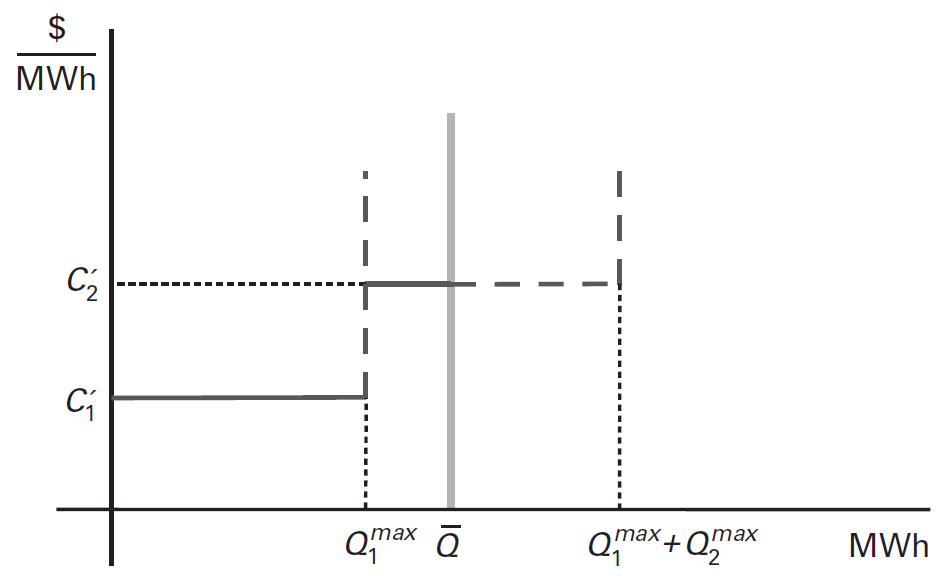
\includegraphics[scale=.3]{figure/dispatching_2.png}
    \caption{Despachamento Ótimo quando $q_1^{max},q_2^{max}<\overline{Q}$}
    \label{fig:dispatching_2}
\end{figure}

\section{Ordem de Mérito}
Os resultados discutidos acima são facilmente generalizáveis por indução para $i>2$ usinas. Isto é, dado que podemos ordenar as usinas em termos de eficiência (custo marginal), sem perda de generalidade, faça com que:
\[ c_1(\cdot)<c_2(\cdot)<\hdots<c_I(\cdot) \]

Teremos então que para uma dada carga exógena, as firmas mais eficientes serão ativadas, em ordem, até atenderem a carga $\overline{Q}$ ou alcançarem sua capacidade máxima.

\section{Custo Marginal do Sistema}
Repare que, no caso geral em que temos $I$ usinas, o Lagrangiano pode ser escrito como:
\[\mathcal{L}=\sum_{i=1}^Ic_i(q_i)+\mu\left(\sum_{i=1}^Iq_i-\overline{Q}\right)+\sum_{i=1}^I\lambda_i(-q_i) + \sum_{i=1}^{I}\lambda_{I+i}(q_i-q_i^{max})\]
Mais ainda, note que:
\[\frac{\partial\mathcal{L}}{\partial\overline{Q}}=-\mu\]
Ou seja, $\mu$ representa o custo que o monopolista (ou planejador) deve pagar \textit{na margem} para produzir a última (ou próxima) unidade marginal de eletricidade que atende à carga exógena $\overline{Q}$. Por este motivo, $\mu$ é chamado de Custo Marginal do Sistema.

Podemos repensar o resultado comentado da ordem de mérito com este conceito em mente. De forma geral, resolvendo o problema de otimização com o Lagrangiano acima, teremos 3 possibilidades para o valor de $c_i'(q_i)$:
\begin{align*}
     c_i'(q_i) =\begin{cases}
        -\mu+\lambda_i>-\mu&\text{caso $\lambda_{i}>0$ e $\lambda_{i+I}=0$} \\
        -\mu&\text{caso $\lambda_{i}=0$ e $\lambda_{i+I}=0$} \\
        -\mu-\lambda_{i+I}<-\mu&\text{caso $\lambda_{i}=0$ e $\lambda_{i+I}>0$}
    \end{cases}  
\end{align*}
De forma análoga aos exemplos com apenas duas usinas, poderemos concluir que a resposta ótima da usina $i$ é tal que:
\begin{align*}
    q_i^*=\begin{cases}
        q_i^{max} & \text{caso $c_i'(q_i)<-\mu$}\\
        \omega \in(0,q_i^{max}) & \text{caso $c_i'(q_i)=-\mu$}\\
        0 & \text{caso $c_i'(q_i)>-\mu$}
    \end{cases}
\end{align*}
Repare que essa intuição está em perfeito acordo com a ordem de mérito.

\section{Problema do Planejador Central}
Se flexibilizarmos a hipótese de que $\overline{Q}>0$ é exógeno e fixo, temos que a equivalência entre o Problema do Monopolista e o Problema do Planejador Central deixa de valer. Entretanto, as similaridades entre ambos problemas é notável em virtude da linearidade do problema. Assuma, sem perda de generalidade, que existam $N$ consumidores e que $U(q^1,\hdots,q^N)=\sum_{n=1}^Nu^n(q^n)$. Podemos escrever o Problema do Planejador Central como:
\begin{align*}
    \max_{\substack{q_1,\hdots,q_I\in\mathbb{R}\\q^1\hdots q^N\in\mathbb{R}}}&\quad \sum_{n=1}^Nu^n(q^n) - \sum_{i=1}^Ic_i(q_i)\\
    \text{s.a}&\quad \sum_nq^n=\sum_iq_i\\
    &\quad 0\le q_i \le q_i^{max},\quad \forall i=1,\hdots,I\\
    &\quad 0\le q^n \le q^{n^{max}},\quad \forall n=1,\hdots,N
\end{align*}
Implicando o seguinte Lagrangiano: 
\begin{align*}
    \mathcal{L}=\sum_ic_i(q_i)-\sum_nu^n(q^n)+\mu\left(\sum_iq_i-\sum_nq^n\right)&+\sum_i\lambda_i(-q_i) + \sum_i\lambda_{I+i}(q_i-q_i^{max})\\
    &+\sum_{n}\gamma_n(-q^n) + \sum_n\gamma_{N+n}(q^n-q^{n^{max}})
\end{align*}
Segue, de forma exatamente análoga à seção anterior, que:
\begin{align*}
    q^{n^*}=\begin{cases}
        q^{n^{max}} & \text{caso $u^{n'}(q^n)>\mu$}\\
        \eta \in(0,q^{n^{max}}) & \text{caso $u^{n'}(q^n)=\mu$}\\
        0 & \text{caso $u^{n'}(q^n)<\mu$}
    \end{cases}
\end{align*}
Ou seja, a carga do sistema segue funções de reação similares às de oferta de eletricidade e, destarte, deve atender à ordem de mérito de forma que os agentes com maior utilidade marginal são supridos primeiro, em ordem.
\chapter{Despacho Ótimo no Tempo}
\localtableofcontents 

Este capítulo é baseado nas notas de aula do curso, ministrado em 10/08/2023, e nas informações do Capítulo~7 de \textcite{cretì_fontini_2019}.

\section{Fundamentos}
Alguns conceitos serão fundamentais para o compreendimento da dimensão temporal do consumo de eletricidade. O primeiro deles é o de fator de capacidade (\textit{Capacity Factor}), já o segundo é a duração de carga (\textit{Load Duration}).
\begin{defin}[Fator de Capacidade]
    A fração de uma quantidade total de tempo em que existe uma determinada quantidade de carga ou geração sobre o sistema.
\end{defin}
\begin{defin}[Duração de Carga]
    O inverso da função de densidade acumulada da carga em relação ao fator de capacidade em um intervalo de tempo específico.
\end{defin}
Naturalmente, ambos conceitos estão intrinsecamente ligados. Tome, por exemplo, a Figura~\ref{fig:carga}, na qual está exemplificada a carga horária sobre o sistema ao longo de um ano inteiro. Se fosse de interesse exprimir a proporção do tempo em que o sistema está sobre determinado nível de carga, chegaríamos então na Figura~\ref{fig:load}.

\begin{figure}[t]
    \centering
    \begin{subfigure}{\textwidth}
        \centering
        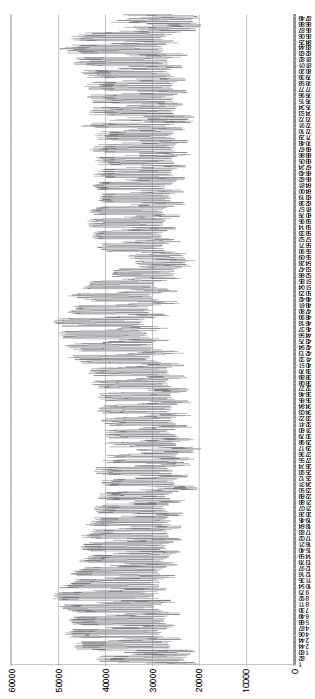
\includegraphics[scale=.5,angle=-90]{figure/carga.png}
        \caption{Exemplo de carga horária sobre o sistema}
        \label{fig:carga}
    \end{subfigure}\\
    \begin{subfigure}{\textwidth}
        \centering
        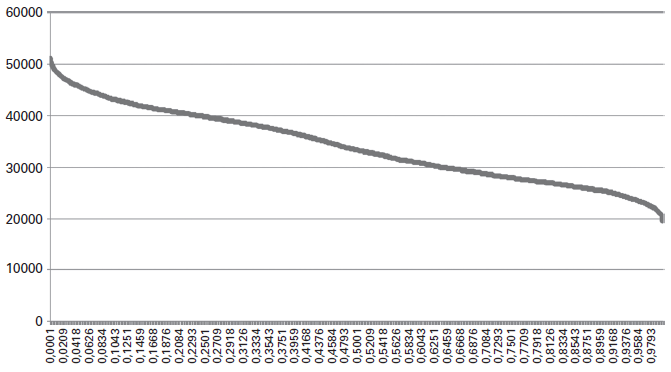
\includegraphics[scale=.5]{figure/load.png}
        \caption{Duração de Carga}
        \label{fig:load}
    \end{subfigure}
    \caption{Relação entre Duração de Carga e Fator de Capacidade}
    \subcaption*{\footnotesize \textit{Nota:} O eixo vertical de ambas figuras representa o total de carga em MWh sobre o sistema. No Painel (a) o eixo horizontal representa as horas do ano, já no Painel (b) representa o fator de capacidade}
\end{figure}  

Da definição a duração de carga temos a ideia de probabilidade - ou densidade acumulada. Esse conceito é importante, pois é uma das principais formas de como ler a Figura~\ref{fig:load}. De forma analítica, temos que: 
\[F(cf) = \{\omega | P(X\leq \omega) = cf\}\]
onde $F(\cdot)$ é a função duração de carga, $X$ é uma variável aleatória representativa da carga sobre o sistema e $cf$ é o fator de capacidade.

\section{Propriedades da Função Custo}
Considere a seguinte forma simplificada de uma função custo (total), onde há uma componente de custo fixo ($FC_i$) e outra de custo variável ($c_i'q_i$):
\[c_i(q_i)=FC_i+c_i'q_i\]

Suponha que ela exprima o custo por hora. Ademais, suponha que a usina $i$, cuja capacidade (por hora) é $q_i^{max}$, produz um total de energia por ano $yq_i = q_i^{max}\cdot h_i$, onde $0\le h_i\le8760$. Ora, repare que $h_i$ denota o a quantidade de tempo efetiva durante a qual a usina $i$ está produzindo ao longo do ano, o que pode ser expresso em termos de fator de capacidade como $h_i=cf_i\cdot8790$. Finalmente, suponha que $FC_i=hRC_i\cdot q_i^{max}$, onde $hRC_i$ denota o custo de aluguel por hora da usina $i$. Podemos, então, reescrever a função acima como:
\[yc_i(q_i)=hRC_i\cdot q_i^{max}\cdot8760+c_i'\cdot q_i^{max}\cdot cf_i\cdot8760\]

Seguem duas definições importantes para o argumento dos próximos capítulos:
\begin{defin}[Custo Médio de Energia - CME]
    O custo de geração por unidade de energia produzida ou produzível.
\end{defin}
Neste exemplo acima, é imediato calcular o CME:
\[CME \equiv \frac{yc_i}{yq_i} = \frac{hRC_i}{cf_i}+c_i'\]
\begin{defin}[Custo Médio de Capacidade - CMC]
    O custo de geração por unidade de capacidade instalada ou instalável.
\end{defin}
Da mesma forma, o CMC é dado por:
\[CMC\equiv \frac{yc_i}{q_i^{max}\cdot8790} = hRC_i+c_i'\cdot cf_i\]
Uma representação gráfica para a equação acima é dada na Figura~\ref{fig:cmc}, considerando $c_i'=\alpha$ e $hRC_i=FC_3$, por exemplo.
\begin{figure}[t]
    \centering
    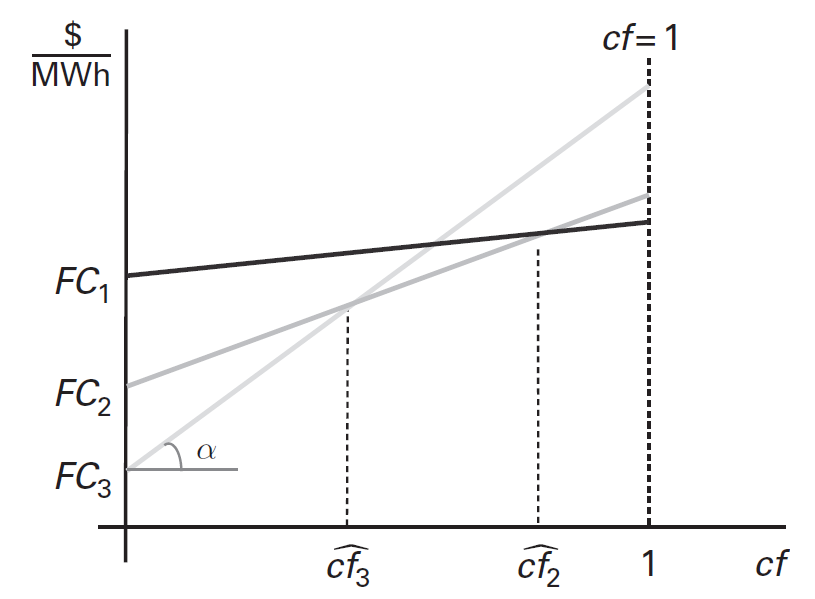
\includegraphics[scale=.3]{figure/cmc.png}
    \caption{Custo Médio de Capacidade - CMC}
    \label{fig:cmc}
\end{figure}

\section{Problema do Planejador Central em T Horas}
Podemos pensar a dimensão temporal do problema a partir dos dados. Lembre que a cuva de Duração de Carga pode ser interpretada como a probabilidade de se encontrar um determinado valor $\overline{Q}$ - associada à um fator de capacidade. Portanto, podemos pensar que um problema estático é resolvido em cada instante de tempo e, destarte, é natural inferir que em uma estrutura energética que atende à ordem de mérito o número em operação vai depender do fator de capacidade de cada instante $t$. É isso o que vamos discutir nessa seção.

De forma geral, podemos ligar vários dos conceitos que vimos até agora tal qual exposto na Figura~\ref{fig:welfare_time}. Nela, supomos um sistema representado pela curva de Duração de Carga descrita no canto direito superior da figura. Note que o sistema sempre utiliza ao menos $M^{min}$ e, em contrapartida, opera com no máximo $M^{max}$. Supomos também que existem apenas três usinas - $A$, $B$ e $C$ - e que o custo marginal é crescente por usina, mas que o oposto vale para os custos fixos ($FC_i$). A solução do problema de maximização do bem-estar que segue a ordem de mérito fornecido pelos custos marginais também é chamado de despacho econômico.

\begin{figure}
    \centering
    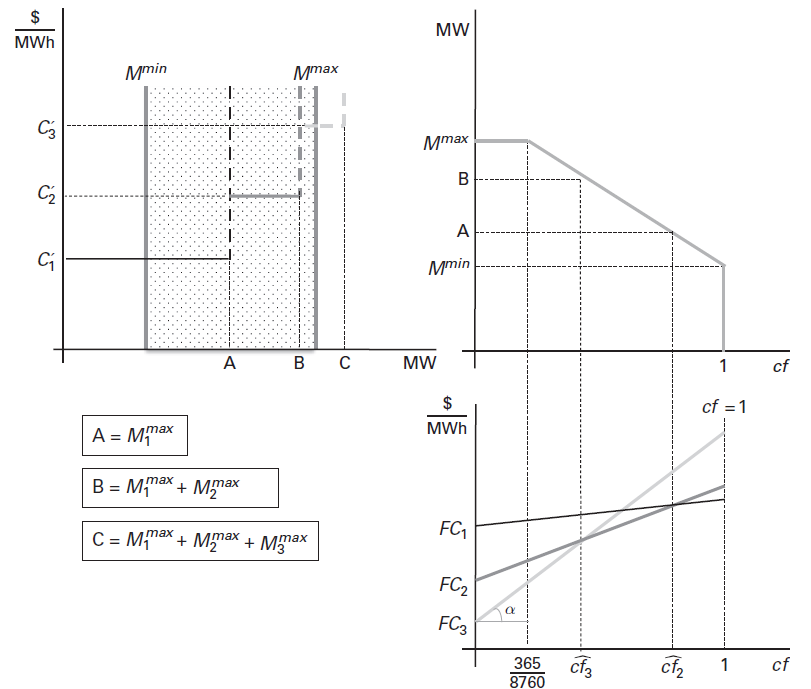
\includegraphics[scale=.5]{figure/economic_dispatch.png}
    \caption{Problema de Maximização de Bem-Estar ao Longo do Tempo}
    \label{fig:welfare_time}
\end{figure}

\begin{defin}[Despacho Econômico]
    A utilização/ativação das usinas é feito de acordo com a ordem de mérito fornecida pelos custos marginais.
\end{defin}

Note que, seguindo o despacho econômico, quando a carga está no mínimo apenas a planta $A$ é acionada. Isso muda exatamente no ponto em que a carga é tal que a usina $A$ não é capaz de suprir a demanda energética ou, alternativamente, em que o fator de capacidade implica o CMC da próxima unidade de eletricidade ser menor na usina $B$ que na usina $A$. 

Mais ainda, repare que a área entre o intervalo de carga gerado (no máximo) por uma usina e o eixo horizontal equivale ao total de energia gerado por ela - tal qual exemplificado na Figura~\ref{fig:tot_energy}. Mais ainda, a energia (potencialmente) gerada pela usina de menor custo marginal é denominada \textbf{carga base} (\textit{base load}), euqnato a energia grada pela usina menos eficiente é denominada \textbf{carga de pico} (\textit{peak load}). A energia gerada entre a carga base e carga de pico é denominada, por sua vez, de \textit{mid-merit}.

\begin{figure}
    \centering
    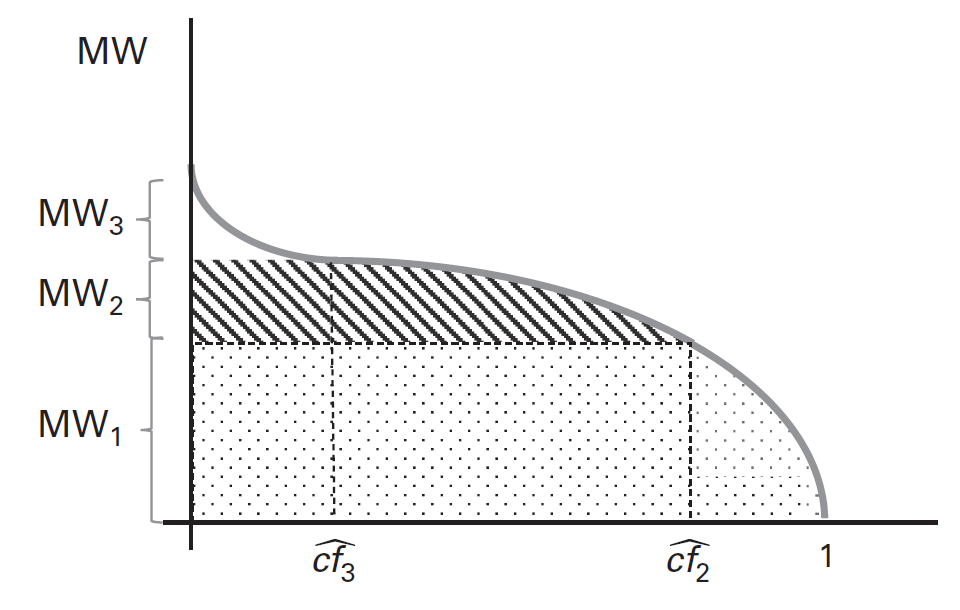
\includegraphics[scale=.25]{figure/tot_energy.png}
    \caption{Total de Eletricidade Gerado por Usina}
    \label{fig:tot_energy}
\end{figure}

\section{Desligamento de Carga Otimizado}
Note que no exemplo descrito na subseção anterior é assumido $M^{max}<A+B+C$ i.e. que a capacidade de geração é maior que a carga máxima do sistema - hipótese que flexibilizaremos aqui. 

Para responder o que acontece nesse caso de claro desiquilíbrio, lembre do Problema do Planejador Central descrito na seção anterior e da simetria de seus resultados com o Problema do Monopolista. Visto que a teoria é perfeitamente análoga, podemos demonstrar que existirá uma "ordem de mérito" para consumidores também, ordenados por suas utilidades marginais. Destarte, consumidores com maior utilidade marginal serão supridos primeiro, seguindo a "ordem de mérito" sucessivamente.

Enquanto a carga for compatível com a capacidade do sistema é trivial observar que todos os consumidores serão atendidos. Entretanto, quando chegamos na carga de pico e, potencialmente, na carga máxima, suposta a partir de agora $M^{max}>A+B+C$, alguém deverá deixar de ser atendido. Resta, portanto, a pergunta sobre como determinar esse processo de forma a maximizar bem-estar. Ora, isso é facilmente respondido, novamente, pelo Problema do Planejador Central. Fixe um instante $t$ de tempo e suponha que neste instante a carga total demandada $\sum_nq^n\equiv Q^N$ é maior que a capacidade do sistema. O problema pode ser escrito como:
\begin{align*}
    \max_{Q^N\in\mathbb{R}}&\quad U(Q^N) - \sum_{i=1}^Ic_i(q_i)\\
    \text{s.a}&\quad Q^N=\sum_iq_i\\
    &\quad 0\le q_i \le q_i^{max},\quad \forall i=1,\hdots,I\\
    &\quad 0\le Q^N \le Q^{{N^{max}}}\equiv M^{max}\\
    &\quad M^{{N^{max}}}>\sum_iq_i^{max}
\end{align*}
Implicando Lagrangiano:
\begin{align*}
    \mathcal{L}=\sum_{i=1}^Ic_i(q_i)-U(Q^N)+\mu(Q^N-\sum_iq_i)+\lambda(\sum_iq_i^{max}-M^{{N^{max}}})
\end{align*}
Implicando a seguinte restrição de estacionariedade:
\begin{align*}
    \frac{\partial\mathcal{L}}{\partial Q^N} = -U'(Q^N) + \mu - \lambda = 0
\end{align*}
Ora, como a restrição referente à $\lambda$ é inativa, por definição, temos que $\lambda=0$, implicando $U'(Q^N) = \mu $. Seja $Q^{N^*}\equiv \Tilde{M}$ a solução do problema acima. A carga desligada (não servida) ótima pode ser escrita, portanto, como $M^{max}-\Tilde{M}$. Segue uma importante definição:
\begin{defin}[Valor da Carga Perdida - \textit{Value of Lost Load}, VOLL]
    O valor da carga referente a se ter uma unidade marginal a mais de capacidade instalada no sistema. 
\end{defin}
Note que o VOLL indica o valor que o consumidor está disposto a pagar para ter uma unidade a mais de energia i.e. o VOLL é expresso como $\mu$ no problema descrito acima (ver Capítulo~\ref{kkt}). Seguem mais duas definições importantes:
\begin{defin}[Expectativa de Carga Perdida, \textit{Loss of Load Expectation}, LOLE]
    O número de unidades de tempo em um dado período (por exemplo, horas do ano) em que se espera que a carga seja perdida.
\end{defin}
\begin{defin}[Probabilidade de Perda de Carga, \textit{Loss of Load Probability}, LOLP]
    A probabilidade de que em um determinado momento haverá perda de carga.
\end{defin}
Ora, se essa carga perdida representa um custo-oportunidade para os consumidores, ela pode ser expressa em unidades monetárias. Portanto, é possível recuperar uma "função dano" ($DF$) quantificando o valor econômico da expectativa de energia não servida:
\begin{align*}
    DF= LOLE\cdot \left(M^{max}-\Tilde{M}\right) \cdot VOLL 
\end{align*}

A Figura~\ref{fig:shedding} indica a interação dessa função dano com o equilíbrio discutido anteriormente. Note que no momento em que fator de capacidade é tal que o valor econômico da expectativa de energia não servida de uma unidade a mais de eletricidade é menor que o custo de produzi-la, cessa-se a geração de energia (ao nível $\Tilde{M}<M^{max}$).    

\begin{figure}
    \centering
    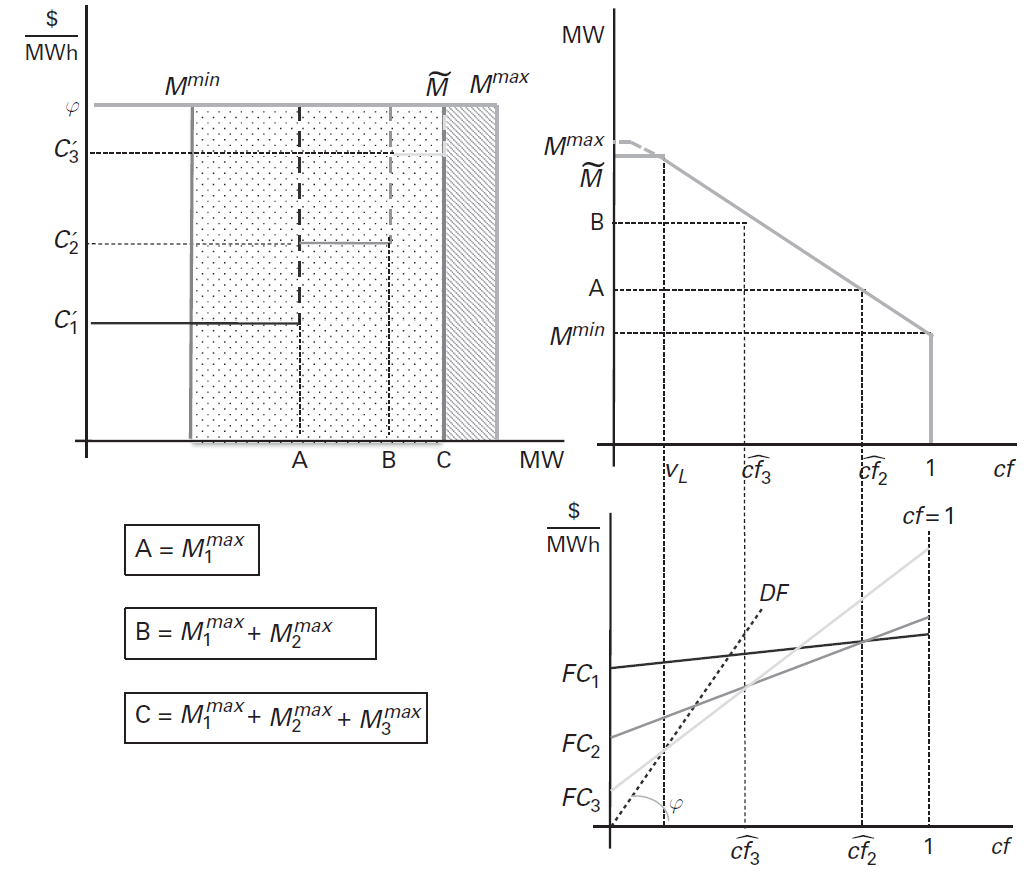
\includegraphics[scale=.4]{figure/shedding.png}
    \caption{Problema de Maximização de Bem-Estar ao Longo do Tempo com Desligamento de Carga}
    \label{fig:shedding}
\end{figure}

\chapter{Problema Descentralizado de Despacho Ótimo}
\localtableofcontents 

O conteúdo deste capítulo é uma versão altamente simplificada dos argumentos passados no Capítulo~10 de \textcite{cretì_fontini_2019}. Ainda mais que nos outros capítulos dessas notas de aula, aqui é recomendado uma leitura do material original para melhor compreensão dos conceitos.

\section{Problema da Firma Competitiva}
O problema em questão se resumo a maximizar o lucro, desconsiderando as outras características do mercado. Portanto, para uma firma $i$ qualquer, esse problema pode ser escrito como:
\begin{align*}
    \max&\quad \pi_i=p_iq_i-c_i(q_i)\\
    \text{s.a.}&\quad 0\le q_i\leq q_i^{max}
\end{align*}
Implicando Lagrangiano:
\begin{align*}
    \mathcal{L} = c_i(q_i)-p_iq_i + \lambda_{1i}(q_i-q_i^{max}) - \lambda_{2i}q_i
\end{align*}
A condição de estacionariedade (CPO) implica:
\begin{align*}
    p_i = c_i'(q_i)+\lambda_{1i}-\lambda_{2i}
\end{align*}
Em um equilíbrio de mercado haverá um preço único para o bem produzido (eletricidade). Portanto, podemos reescrever a condição acima de forma mais geral como:
\[p=c_i'(q_i)+\lambda_{1i}-\lambda_{2i}, \forall i\]
Esse resultado é poderosíssimo, pois nos compra algumas propriedades muito importantes. Em específico, é possível demonstrar que valerá ordem de mérito mesmo no equilíbrio descentralizado (veja \textcite{cretì_fontini_2019} Seção 10.2).

\section{Problema do Consumidor}
O consumidor quer maximizar sua utilidade descontada dos custos associados à compra dos bens. Poderíamos escrever esse problema através de uma restrição orçamentária (tal qual padrão em economia). Entretanto, como estamos considerando utilidade em unidades monetárias \hl{(vou verificar com o professor o porquê disso...)}, podemos simplificar o problema do consumidor $j$ para:
\begin{align*}
    \max&\quad u^j(q^j)-p^jq^j\\
    \text{s.a.}&\quad 0\le q^j\le q^{j^{max}}
\end{align*}
Implicando Lagrangiano:
\begin{align*}
    \mathcal{L} = p^jq^j - u^j(q^j) + \lambda_{1}^j(q^j-q^{j^{max}}) - \lambda_{2}^jq^j
\end{align*}
A condição de estacionariedade (CPO) implica:
\begin{align*}
    p^j = u^{j'}(q^j)-\lambda_{1}^j+\lambda_{2}^j
\end{align*}
O mesmo argumento de unicidade de preço vale para o problema do consumidor e gera conclusão similar i.e. validade da ordem de mérito onde os consumidores com maior utilidade marginal são servidos primeiro.

\section{Equilíbrio de Mercado}
Tal qual padrão em economia, o equilíbrio de mercado é definido como o par de preço $P^*$ e quantidade $Q^*$ tal que a oferta e demanda de energia se igualam. A forma mais imediata de se recuperar esses valores é igualando os preços encontrados nas duas seções anteriores.

\begin{defin}[Preço Marginal do Sistema]
    O preço de equilíbrio no mercado de eletricidade
\end{defin}

Se assumirmos funções lineares e afins (tal qual padrão nesse curso), teremos um total de 4 tipos de equilíbrio, exemplificados na Figura~\ref{fig:eq}. A fins de clarificação, o equilíbrio c) é tal que o preço $P^*$ é a linha pontilhada inferior, já no equilíbrio d) a quantidade $Q^*$ é a linha pontilhada à direita.

\begin{figure}
    \centering
    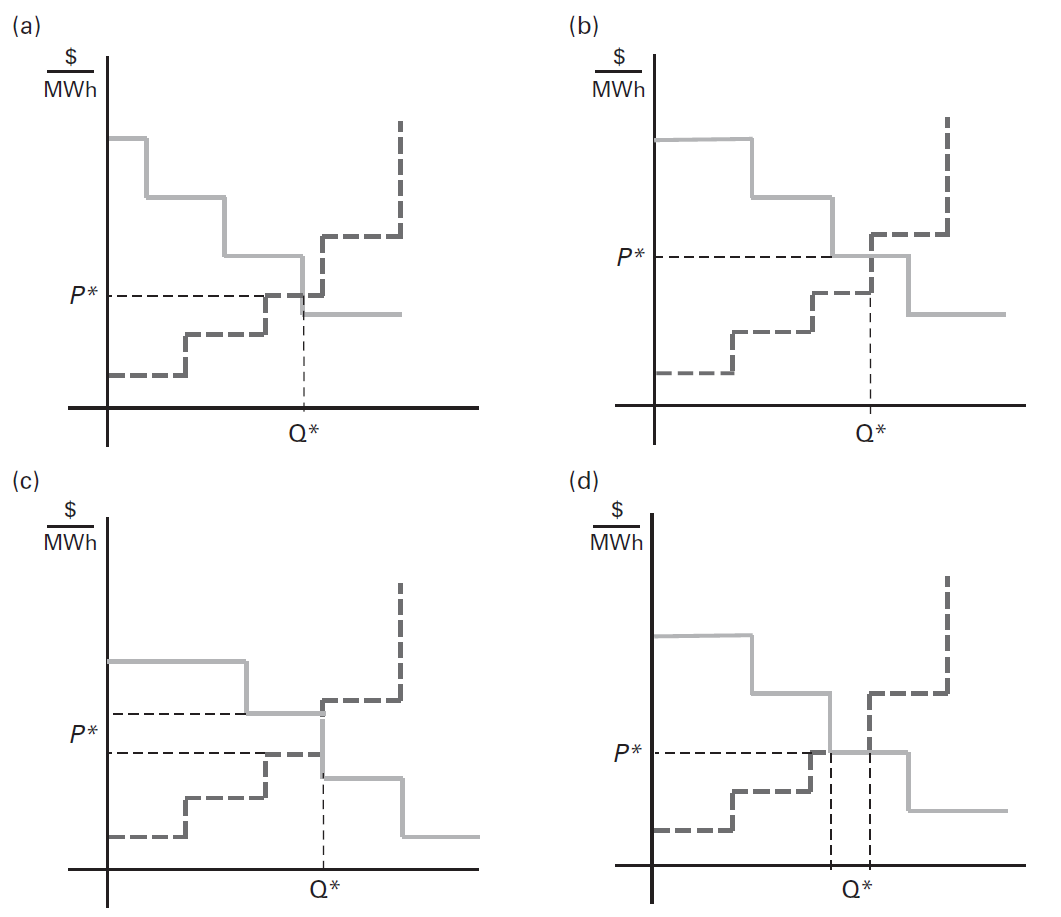
\includegraphics[scale=.35]{figure/eq.png}
    \caption{As Quatro Possibilidades de Equilíbrio de Mercado}
    \label{fig:eq}
\end{figure}

\subsection{Equivalência entre Problemas}
Note que os resultados do Problema da Firma, Problema do Consumidor e do Problema do Planejador Central são extremamente parecidos. Em específico note que $\mu$ age como o análogo do preço no problema do planejador central.

Essa semelhança não é surpreendente e decorre do chamado "Primeiro Teorema do Bem-Estar", que enuncia as condições (aqui atendidas) para que o equilíbrio de mercado competitivo seja idêntico ao equilíbrio do planejador central - ou do monopolista perfeitamente regulado (sem assimetria de informação).

\begin{teo}[Primeiro Teorema do Bem-Estar]
    Sob competição perfeita, o equilíbrio de mercado competitivo é Pareto eficiente i.e. idêntico ao equilíbrio derivado do problema do planejador central maximizador de bem-estar social.
\end{teo}


\chapter{Falhas de Mercado}
\localtableofcontents 

Este capítulo é baseado nas notas de aula do curso, ministrado em 12/08/2023, e nos capítulos 12 (principal) e 13 de \textcite{cretì_fontini_2019}.

Por definição, uma firma tem poder de mercado se ela é capaz de discriminar preços total ou parcialmente. A forma como isso é feito pode mudar, mas essa característica permanece sempre. Por exemplo, um monopolista escolhe o preço e quantidade em que vende o produto diretamente, enquanto oligopolistas impactam o preço de equilíbrio estrategicamente via mudança nas quantidades ofertadas.

Nesta seção vamos discutir como competição imperfeita altera os resultados dos últimos capítulo e em que condições isso pode representar um problema para os procedimentos do mundo real.

\section{Competição Imperfeita}
Existem dois modelos principais modelos utilizados para estudar o tópico de competição imperfeita: Cournot e Bertrand. Ambos são chamados "jogos estratégicos", ou seja, as firmas se comportam como atores em um jogo no qual sempre preveem o comportamento da outra parte (assume-se racionalidade). Em todos esses modelos, tal qual apresentados aqui, são assumidos bens homogêneos.

\subsection{Modelo de Cournot}
Esse é o modelo prototípico de oligopólios. Aqui não será o foco derivar completamente o modelo e seus resultados (será coberto nas monitorias), apenas discutir as principais intuições.

Neste modelo cada firma opera como um monopolista na demanda residual das outras. Tome uma firma $i$, por exemplo. Ela escolherá uma quantidade para produzir, entendendo que sua escolha alterará o preço final do bem. Mais ainda, ela não se preocupa em atender a todo mercado, apenas a uma parcela de forma a maximizar seu lucro. 

Durante a escolha dessa quantidade ótima, ela leva em consideração que as demais firmas $-i$ também se deparam com um problema simétrico. Naturalmente, as firmas querem tomar a maior fatia do mercado para elas e, portanto, produzir mais. Entretanto, se todas produzirem muito o preço irá abaixar, não compensando o lucro que poderiam extrair da parcela ótima do mercado.

O resultado dessas forças atrativas e repulsoras de produção é chamado de equilíbrio de Cournot $(P^c,Q^c)$, que, via de regra, é tal que $Q^*>Q^c$ e $P^*<P^c$ onde $(P^*,Q^*)$ é o equilíbrio de mercado competitivo. 
\subsection{Modelo de Bertrand}
Esse é um modelo alternativo, mas igualmente importante e aplicável de monopólios, onde os incentivos são marginalmente diferentes. Ao invés de competirem na demanda residual (e, portanto, quantidades) como no modelo de Cournot, as firmas do oligopólio competem em preços.

Seja um preço fixo inicial $P_0$. Cada firma enfrenta o mesmo jogo (simétrico) e incentivos. A firma $i$ sabe que se abaixar o preço $P_0$ em uma quantidade infinitesimal $\varepsilon>0$ ela tomará todo o mercado para si (não há custos de transação) . Naturalmente, a firma $-i$ responderá abaixando o o preço $P_0$ em $2\varepsilon$, para roubar o mercado todo da firma $i$, e assim sucessivamente. 

O resultado dessa competição de preços é tal que o preço de equilíbrio $P^b$ será igual ao custo marginal da segunda firma mais eficiente i.e. $P^b=C_2'(Q^b)$. Em específico, no caso de um duopólio, esse resultado é idêntico ao de um equilíbrio competitivo.

\section{Leilões}
Leilões são uma das formas possíveis de se organizar um mercado que é interessante, em particular, por possibilitar recuperar preferências e demanda pelo bem comercializado. Esse é um campo enorme dentro de microeconomia e teoria econômica, mas que resumirei em alguns tipos abaixo:
\begin{itemize}
    \item \textbf{Leilões de Primeiro Preço:} Um leilão é realizado onde os apostadores não veem os lances dos seus adversários. O vencedor paga ao leiloeiro o valor de seu próprio lance.
    \item \textbf{Leilões de Segundo Preço:} Um leilão é realizado onde os apostadores veem os lances de seus adversários. Logo, o vencedor, por racionalidade, paga o valor muito próximo do segundo maior lance.
    \item \textbf{Leilões Uniformes:} Um leilão em que tanto oferta e demanda fazem preço. Pessoas escolhem vender um bem e outras escolhem comprá-lo. Desse processo surge um preço, tal qual em equilíbrio competitivo, mas todos entendem que sua decisão influenciará o preço final. Em Leilões Uniformes os "vencedores" irão receber/pagar o mesmo preço, independente do que tenham apostado.
    \item \textbf{Leilões Discriminatórios:} Similares à leilões uniformes, entretanto, cada apostador vencedor pagará o valor equivalente ao seu lance.
\end{itemize}
No contexto de eletricidade, é interessante pensar nessa estrutura de leilões, pois é assim que o processo de concessão de geração de energia costuma acontecer. Vamos, aqui, discutir em detalhe principalmente os últimos dois tipos de leilões e as implicações deles em cenários competitivos e - interessantes à esse capítulo - não-competitivos.

A Figura~\ref{fig:leil_comp} mostra os incentivos das empresas competitivas em ambas modalidades de leilão. Primeiro, note que a firma nunca tem incentivos à desviar do seu custo marginal para baixo pois, caso ganhe, ela estará pior do que caso tenha perdido (lucro negativo). Em leilões uniformes, as firmas também não tem incentivo à desviar para cima, pois as vencedoras vão receber o preço da firma marginal (na margem da vitória) independente disso, logo preferem aumentar a probabilidade de vencerem apostando seu custo marginal. Já em leilões discriminatórios, as firmas conseguem prever qual será o preço de equilíbrio e, portanto, as firmas que esperam vencer apostam nesse preço de equilíbrio para maximizar lucro. Portanto, sob mercados competitivos, ambos leilões levam aos mesmos resultados ainda que por mecanismos diferentes

\begin{figure}
    \centering
    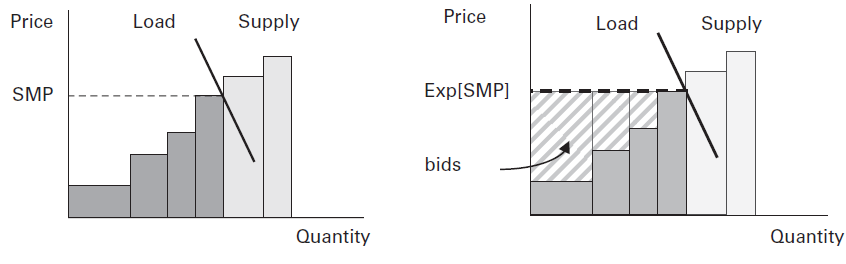
\includegraphics[scale=.5]{figure/leilao_comp.png}
    \caption{Diferenças de Leilões - Mercados Competitivos}
    \subcaption*{\footnotesize \textit{Nota:} A figura da esquerda mostra os incentivos das firmas em um sistema de leilão uniforme, já a figura da direita em um leilão discriminatório.}
    \label{fig:leil_comp}
\end{figure}

A Figura~\ref{fig:leil_ncomp_p}, por outro lado, mostra os incentivos para firmas não competitivas que estão exercendo poder de mercado (competindo) em preços. Note que o argumento anterior é exatamente válido aqui para todas as firmas exceto a marginal. Essa firma, em específico, tem incentivos a mentir e a reportar seu custo marginal apenas um $\varepsilon>0$ menor que a próxima firma na ordem de mérito para extrair lucro máximo. Em leilões discriminatórios, o mesmo argumento também vale para a firma marginal. Para as demais, entretanto, por ser mais difícil inferir o preço de equilíbrio, todas tem incentivo a apostar um pouco mais que seu custo marginal, mas não de forma generalizada à $P^*$ como no caso competitivo.

Caso as firmas compitam em volume, vemos na Figura~\ref{fig:leil_ncomp_p} que todas as firmas tem incentivo a mentir a sobre a quantidade em estoque/a ser entregue. Elas informam um valor menor e, assim, "empurram" a curva de oferta para esquerda, inflando os preços, por sua vez.

\begin{figure}[!b]
    \centering
    \begin{subfigure}{\textwidth}
        \centering
        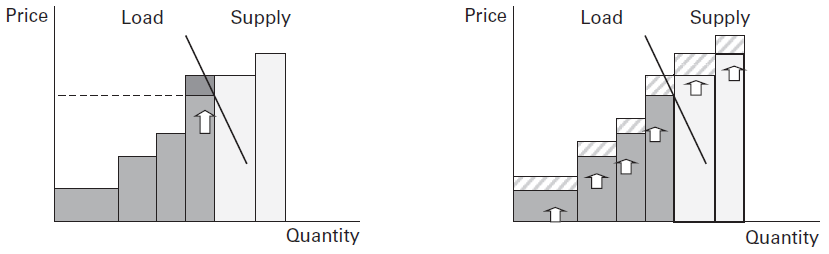
\includegraphics[scale=.5]{figure/leilao_ncomp_a.png}
        \smallskip
        
        \caption{Poder de Mercado em Preços}
        \label{fig:leil_ncomp_p}
    \end{subfigure}
    \smallskip
    
    \begin{subfigure}{\textwidth}
        \centering    
        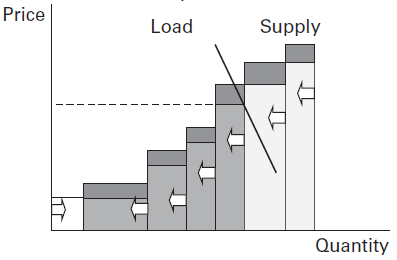
\includegraphics[scale=.5]{figure/leilao_ncomp_b.png}
        \caption{Poder de Mercado em Quantidades}
        \label{fig:leil_ncomp_q}
    \end{subfigure}
    \caption{Caption}
    \label{fig:leil_ncomp}
    \subcaption*{\footnotesize \textit{Nota:} No Painel (a), a figura da esquerda mostra os incentivos das firmas em um sistema de leilão uniforme, já a figura da direita em um leilão discriminatório. Já no Painel (b) a figura é referente a leilões uniformes, visto que discriminatórios com poder de mercado em volume é pouco sustentável do ponto de visto de incentivos.}
\end{figure}

\section{Medindo Competitividade}
Durantes as aulas foram apresentados dois índices comumente utilizados para medir o grau de competitividade de mercados: o \textit{Herfindahl-Hirschmann Index} (HHI); e o \textit{Pivotal Supplier Index} (PSI). Além das diferenças metodológicas, é importante notar que o HHI é utilizado em uma pluralidade de contextos, enquanto o PSI é específico da análise do setor de energia. No Capítulo 13 de \textcite{cretì_fontini_2019} também são discutidas outras possíveis formas de se mensurar concentração de mercados.

\subsection{\textit{Herfindahl-Hirschmann Index} (HHI)}
O HHI é definido como a soma dos quadrados dos \textit{market-shares} de $n$ empresas em um determinado setor i.e.:
\begin{align*}
    HHI=\sum_{i=1}^ns_i^2
\end{align*}
onde $s_i$ denota o \textit{market-share} da firma $i$.

É comum usar \textit{market-shares} expressas em termos percentuais para calcular o HHI ou, alternativamente, multiplicá-lo por 10.000. A Divisão Antitruste do Departamento de Justiça nos Estados Unidos (DOJ) usa os seguintes níveis:
\begin{itemize}
    \item $HHI<1000$ denota um mercado não-concentrado;
    \item $HHI\in(1000,1800]$ denota um mercado com baixa concentração;
    \item $HHI>1800$ denota um mercado concentrado (pouco competitivo)
\end{itemize}
No entanto, usar o HHI para avaliar a concentração em mercados de energia pode produzir resultados enganosos. Nesses mercados, como vimos, as fábricas normalmente têm restrições de capacidade. Isso implica diferentes estruturas de mercado podendo produzir diferentes
HHIs, mas afetando o preço de equilíbrio.

\subsection{\textit{Pivotal Supplier Index} (PSI)}
O PSI foi proposto por \textcite{borenstein1999market} e é uma
tentativa de incorporar o conceito de fornecedor marginal na mensuração do poder de mercado nos mercados de eletricidade. Este indicador examina se um determinado produtor ou usina é “pivotal” i.e. necessário para atender a demanda em um determinado momento, no sentido de que haverá um desligamento de carga sem a presença desta usina. O PSI pode ser definido como a razão de todas as horas (ou diferentes unidades de tempo) em que a usina foi pivotal por um determinado período. Por exemplo, se o período for um ano e a unidade de tempo for horas, o PSI da usina $i$ é:
\begin{align*}
    PSI_i = \frac{\sum_{j=1}^{8760}\mathbbm{1}\left[q^{dj}-\sum_{\substack{f=1\\f\neq i}}^nq_f^{max}\right]}{8760}
\end{align*}
onde $q^{dj}$ denota a carga na hora $j$ e $\mathbbm{1}[\cdot]$ é a função indicadora. Enquanto o HHI é uma medida da concentração geral do mercado, o PSI é uma medida de concentração do excedente de capacidade do sistema, ou seja, a possibilidade de igualar o total
oferta e demanda do sistema em qualquer período de tempo específico. 

Uma conclusão importante deste índice é que é possível que uma usina que não é despachada (esta à direita da curva) é importante para determinar poder de mercado, pois sua remoção do leilão pode implicar geração de usinas pivotais.
\chapter{Investimento Ótimo}
\localtableofcontents 

Este capítulo é baseado nas notas de aula do curso, ministrado em 11/08/2023 e 14/08/2023, e nos capítulos 21 e 22 de \textcite{cretì_fontini_2019}.

A análise deste capítulo é parecida com a dos exercícios de Despacho Ótimo dos capítulos anteriores. Entretanto, flexibilizamos uma hipótese que anteriormente era imposta: capacidade máxima de geração fixa. O propósito deste capítulo é pensar em formas de determinação endógena dessa capacidade.

\section{Problema Centralizado de Investimento Ótimo}
Suponha a existência de uma única tecnologia de geração i.e. todas as usinas possuem o mesmo custo de produção. A maximização deste problema no instante $t$ é dada por:
\begin{align*}
    \max_{M_i^{max},q_i,q^d}&\quad U(q^d) - \sum_{i=1}^nc_i(q_i,M_i^{max})\\
    \textbf{s.a.}&\quad q^d=\sum_iq_i\\
    &\quad q_i\ge0,\forall i\\
    &\quad q_i\le M_i^{max},\forall i
\end{align*}
Implicando o Lagrangiano:
\begin{align*}
    \mathcal{L}=\sum_{i=1}^nc_i(q_i,M_i^{max})-U(q^d)+\mu\left(\sum_iq_i-q^d\right)-\sum_i\lambda_iq_i+\sum_i\lambda_{n+i}(q_i-M_i^{max})
\end{align*}
Implicando as CPOs:
\begin{align*}
    \frac{\partial\mathcal{L}}{\partial q_i}&=c_{i,q_i}+\mu-\lambda_i+\lambda_{n+i}=0\Longleftrightarrow c_{i,q_i} =-\mu-\lambda_{n+i}-\lambda_i,\forall i \\
    \frac{\partial\mathcal{L}}{\partial q^d}&=-U'(q^d)-\mu=0 \Longleftrightarrow  U'(q^d) = -\mu\\
    \frac{\partial\mathcal{L}}{\partial M_i^{max}}&=c_{i,M_i^{max}}-\lambda_{n+i}=0 \Longleftrightarrow c_{i,M_i^{max}}=\lambda_{n+i}, \forall i
\end{align*}
Onde os subscritos em $c_i$ denotam as derivadas parciais. Considerando a solução interna teremos:
\begin{align*}
    \lambda_{n+i}&=c_{i,M_i^{max}},\forall i\\
    \lambda_{n+i}&=(U'(q^d)-c_{i,q_i})\cdot\mathbbm{1}[M_i^{max}=q_i],\forall i
\end{align*}
Igualando as equações e dividindo pelo horizonte de tempo $T$ temos:
\begin{align*}
    \underbrace{\frac{c_{i,M_i^{max}}}{T}}_{hRC_i} = (\underbrace{U'(q^d)}_{VOLL}-\underbrace{c_{i,q_i}}_{c_i})\cdot\underbrace{\frac{\mathbbm{1}[M_i^{max}=q_i]}{T}}_{P(q^d>M_i^{max})\equiv LOLP_i},\forall i
\end{align*}
Onde $hRC_i$ é o custo do aluguel do capital instalado na usina $i$ e VOLL e LOLP são conceitos definidos no Capítulo~3. Ora, então temos que LOLP pode ser definido também (no longo prazo) como:
\begin{align*}
    LOLP_i = \frac{hRC_i}{VOLL-c_i}
\end{align*}
Assim, vemos como é possível definir o nível ótimo de capacidade: A capacidade ótima de longo prazo é aquela que faz LOLP atender à equação acima. Mais ainda, note que $c_i$ é de uma ordem de magnitude muito inferior a $VOLL$ e, portanto, podemos ignorá-la de forma a obter:
\begin{align*}
    LOLP_i\approx \frac{YRC_i}{VOLL}
\end{align*}
Onde $YRC_i$ denota o aluguel anual do capital instalado na usina $i$. A equação acima é normalmente referida como "preço da carga máxima" ou \textit{VOLL-pricing}.

\section{Problema Descentralizado de Investimento Ótimo}
No problema descentralizado o objetivo da firma é maximizar seus lucros. Iremos supor 3 tecnologias, de forma a termos usinas de "carga base", "carga de pico" e \textit{mid-merit}. Mais ainda, note que o preço do produto final dependerá das decisões de produção de todas as firmas conjuntamente.

Vamos começar pelo problema da firma de carga de pico (\textit{peaker}). Note que ela só produz quando $q^d>M_1^{max}+M_2^{max}$, por definição. Mais ainda, essa firma se depara com dois cenários de preços: 1) há desligamento de carga e, portanto, o preço é $\phi=VOLL$, o que ocorre com probabilidade $v_L=LOLP$; e 2) ela é a firma marginal e o preço será o do sistema i.e. $c_3$, ocorrendo com probabilidade $cf_3-v_L$. A receita do 
\textit{peaker} é dada, então, por:
\[\pi_3=\phi v_LM_3^{max}+c_3(cf_3-v_L)M_3^{max}\]
Seus custos dados por:
\[YRC_3M_3^{max}+c_3cf_3M_3^{max}\]
Implicando lucro:
\[\pi_3=(\phi-c_3) v_LM_3^{max}-YRC_3M_3^{max}\]
Analogamente, teremos que os lucros das firmas \textit{mid-merit} e "carga base" (\textit{baseload}) serão dados por, respectivamente:
\begin{align*}
    \pi_2&=(\phi-c_3)v_LM_2^{max}+(c_3-c_2)cf_3M_2^{max}-YRC_2M_2^{max}\\
    \pi_1&=(\phi-c_3)v_LM_1^{max}+(c_3-c_2)cf_3M_1^{max}+(c_2-c_1)cf_2M_1^{max}-YRC_1M_1^{max}
\end{align*}
É imediato perceber que as CPOs do problema individual de cada firma (onde elas maximizam seu respectivo $M_i^{max}$) implicam:
\begin{align*}
    YRC_3&=(\phi-c_3)v_L\\
    YRC_2&=(\phi-c_3)v_L+(c_3-c_2)cf_3\\
    YRC_1&=(\phi-c_3)v_L+(c_3-c_2)cf_3+(c_2-c_1)cf_2
\end{align*}
Tal qual esperado, esses valores são idênticos aos encontrados no problema de minimização de custos (veja Cap. 21 de  \textcite{cretì_fontini_2019}), ou seja, mais uma aplicação do Primeiro Teorema do Bem-Estar - o que é esperado vide a falta de fricções de mercado. A segunda conclusão que temos deste resultado é que, em perfeita concorrência, há lucro econômico 0 ($\pi_i=0,\forall i$) i.e. os investidores perfeitamente repagam seus investimentos.

\section{Mecanismos de Remuneração de Capacidade (CRMs)}
Uma discussão do mundo real relacionada à esse tópico é que os retorno do capital investido no setor de eletricidade (não confundir com lucro econômico) são muito baixos e, portanto, existem poucos incentivos à atores privados investirem o suficiente para chegar-se aos níveis ótimos. Como os Operadores do Sistema prezam pela eficiência do sistema, algum mecanismo para aumentar esses incentivos deve ser criado.

A fins de comparação, considere apenas duas firmas seguindo a lógica do exercício da sessão anterior (\textit{first-best} i.e. mercados perfeitos):
\begin{align*}
    YRC_2&=(\phi-c_2)v_L\\
    YRC_1&=(\phi-c_2)v_L+(c_2-c_1)cf_2
\end{align*}
Abaixo segue um exemplo desses mecanismos. Para uma discussão mais aprofundada veja o Capítulo~22 de \textcite{cretì_fontini_2019}.

\subsection{Teto de Preços}
Se tivermos um teto de preços $\overline{p}$, será possível chegar à alocação ótima de investimentos se eles forem remunerados ao nível ótimo. Suponha um sistema com limitações de capacidade i.e. $M_2^{mis}=M_2^*-M_2^{ins}$, onde $=M_2^*$ é a capacidade ótima, $M_2^{ins}$ a capacidade instalada e $M_2^{mis}$ a capacidade faltante. 

Por causa da falta de capacidade, temos que $v_L^{ins}>v_L^*$. Mais ainda, a existência dessa falta de capacidade é o teto de preços baixo demais i.e. $\overline{p}<\phi$. Repare a mudança na estrutura de lucros implica duas CPOs marginalmente diferentes:
\begin{align*}
    \text{sem teto de preços:}&\quad YRC_2=(\phi-c_2)v_L^*\\
    \text{com teto de preços:}&\quad YRC_2=(\overline{p}-c_2)v_L^{ins}
\end{align*}
Graficamente, essa dinâmica pode ser observada na Figura~\ref{fig:price_cap}. A área tracejada denota a perda de receitas decorrentes do teto de preços, enquanto a área sombreada denota o ganho de receitas decorrentes do teto. Note que:
\begin{figure}
    \centering
    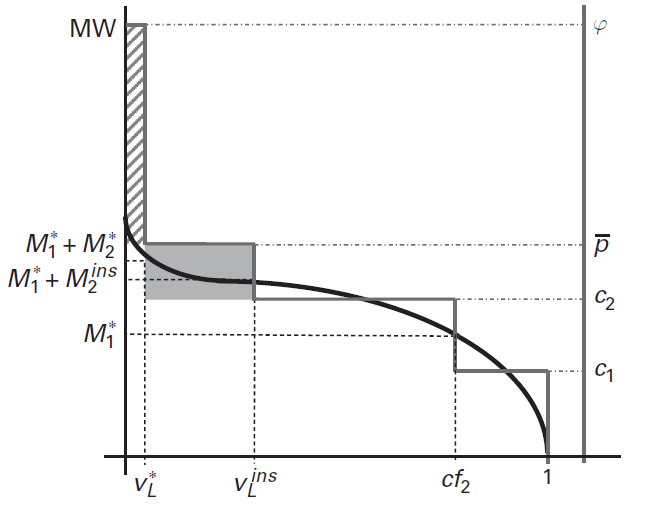
\includegraphics[scale=.4]{figure/price_cap.png}
    \caption{Efeito de Teto de Preços}
    \label{fig:price_cap}
\end{figure}
\begin{align*}
    \underbrace{(\overline{p}-c_2)\cdot(v_L^{ins}-v_L^*)}_{\text{ganhos}} - \underbrace{(\phi-\overline{p})\cdot v_L^*}_{\text{perdas}} <0
\end{align*}
pois, caso contrário, o nível de investimentos seria $M_2^{ins}\ge M_2^*$. Assuma, agora, que o operador paga $k$ por unidade de capital instalado. Com a CRM, o lucro líquido da usina 2 fica:
\begin{align*}
    \overline{\pi_2} =(\overline{p}-c_2)v_L^{ins}M_2^{ins} + kM_2^{ins} - YRC_2M_2^{ins}
\end{align*}
Resta perguntar, então, qual o nível $k$ que maximiza o bem-estar. Ora, é fácil intuir que se remunerarmos a firma pela sua perda de receitas decorrente do teto de preços, a alocação será a ótima. Analiticamente, seja $k = (\phi-\overline{p}) v_L^*-(\overline{p}-c_2)(v_L^{ins}-v_L^*)$. Temos então que:
\begin{align*}
    \overline{\pi_2}(M_2^{ins}) &=(\overline{p}-c_2)v_L^{ins}M_2^{ins} + [(\phi-\overline{p}) v_L^*-(\overline{p}-c_2)(v_L^{ins}-v_L^*)]M_2^{ins} - YRC_2M_2^{ins}\\
    &=(\phi-\overline{p}) v_L^*M_2^{ins} - YRC_2M_2^{ins}\\
    &=\pi^*(M_2^{ins})
\end{align*}
Note que, maximizando em $M_2^{ins}$, o resultado da otimização de lucro levará à mesma alocação de capacidade do ótimo i.e. na ausência de teto de preços. Considerações sobre a firma \textit{baseload} podem ser vistas no Capítulo~22 de \textcite{cretì_fontini_2019}.
\chapter{Transmissão Elétrica}
\localtableofcontents 

Este capítulo é baseado nas notas de aula do curso, ministrado em 14/08/2023 e 16/08/2023, e no capítulo 14 de \textcite{cretì_fontini_2019}.

Até o momento ignoramos completamente o aspecto de transmissão do nosso modelo de despacho ótimo, no sentido que sempre assumimos implicitamente que a transmissão era eficiente e capaz de atender tanto demanda quando oferta de eletricidade. A partir deste momento, consideramos essas restrições de transmissão no modelo.

\section{Despacho Ótimo com Restrições de Transmissão e Preços Nodais}
Adicionar a rede de transmissão implica perguntar como essa rede deve ser precificada. O modelo desta sessão visa explicar esse ponto. Segue uma importante definição:
\begin{defin}[Preços Nodais]
    São os preços que permitem atingir, de forma descentralizada, a solução do problema de despacho de energia ótimo (na rede) maximizador de bem-estar.
\end{defin}

 Nesse contexto, o despacho ótimo de um sistema é a quantidade líquida que deve ser injetada e retirada em cada nó de forma a maximizar o bem-estar social, para uma determinada carga e características técnicas, econômicas e locacionais da geração e transmissão de energia. Portanto, o despacho ótimo representa a alocação que seria decidida por um OS benevolente, perfeitamente informado e exclusivamente preocupado com a eficiência do sistema, mas livre de qualquer preocupação distributiva.

Nesse modelo existe a suposição implícita que todas as usinas no
mesmo nó são pagas o preço uniforme local, associado a esse nó; o mesmo é verdade para a carga. Vamos exemplificar o modelo com o caso mais simples possível.

Suponha a rede seja composta de dois nós tal que em um deles estejam as usinas e no outro os consumidores (carga). Suponha, mais ainda, que só exista uma usina, indexada por $i$. Teremos então que a solução maximizadora de bem-estar é dada por:
\begin{align*}
    \max_{q^d,q_i}&\quad U(q^d)-c(q_i)\\
    \text{s.a.}&\quad q^d=q_i\\
    &\quad q_i\le k^{max}\\
    &\quad 0\le q_i\le q_i^{max}\\
    &\quad 0\le q^n \le q^{n^{max}}
\end{align*}
Implicando o seguinte Lagrangiano:
\begin{align*}
    \mathcal{L} = c(q_i)-U(q^d)+\mu(q_i-q_d)+\chi(q_i-k^{max}) - \lambda_1q_i + \lambda_2(q_i-q_i^{max}) - \lambda_3q^n + \lambda_4(q^n-q^{n^{max}})
\end{align*}
Implicando as CPOs:
\begin{align*}
    \frac{\partial\mathcal{L}}{\partial q_i} &= c'(q_i) +\mu +\chi -\lambda_1+\lambda_2 = 0 \Rightarrow -\mu = c'(q_i)+\chi-\lambda_1 + \lambda_2 \\ 
    \frac{\partial\mathcal{L}}{\partial q^d} &= - U'(q^d) - \mu -\lambda_3+\lambda_4=0 \Rightarrow -\mu = U'(q^d) + \lambda_3-\lambda_4
\end{align*}
E condições de frouxidão complementar:
\begin{align*}
    \mu(q_i-q_d)=\chi(q_i-k^{max}) =\lambda_1q_i =\lambda_2(q_i-q_i^{max})=0
\end{align*}
Além das factibilidades primais e duais. Note, inclusive, que só há congestionamento na transmissão se $q_i=k^{max}$, implicando $\chi>0$. Portanto, $\chi$ representa o valor da linha de transmissão entre os dois nós. Mais ainda, a linha de transmissão só tem valor econômico se houver congestionamento. Desta proposição inferimos que na ausência de congestionamento, teremos CPOs idênticas ao problema visto no Capítulo~2, levando, portanto, a resultados idênticos.

Repare que o problema discutido acima é referente ao planejador central. Naturalmente, sabemos que em um mercado perfeitamente competitivo valerá o Primeiro Teorema do Bem-Estar, implicando equivalência de alocações sob $p=c'(q_i^*)$, na solução interior. Entretanto, conforme discutido anteriormente, caso exista congestionamento na transmissão teremos 
\[p=c'(q_i^*)+\chi\] 
a definição analítica do preço nodal. Logo, se existem diferentes preços entre diferentes nós, sabemos que há congestionamento no sistema.

\section{Múltiplos Nós}
Pode parecer imediata a extensão do exemplo de dois nós, visto na seção anterior, para o caso de múltiplos nós. Isso não é verdade, entretanto, em virtude das características físicas do processo de transmissão de energia - nomeadamente, das chamadas Leis de Kirkoff.

Aqui, resolverei o caso de uma rede com 3 nós - que pode ser mais facilmente generalizado em diferentes contextos. Suponha uma rede na qual cada nó produz e demanda eletricidade em diferentes quantidades com diferentes tecnologias. 

As redes estudadas nesta seção formam um "loop". Esse tipo de configuração é referido como "malha". Seja $f_{j,k}$ o fluxo de eletricidade entre quaisquer nós $j$ e $k$. Suponha que a malha seja tal qual um triângulo equilátero. 

\subsection{Caso Específico}
A Figura~\ref{fig:3_nodes} denota o exemplo graficamente.
\begin{figure}
    \centering
    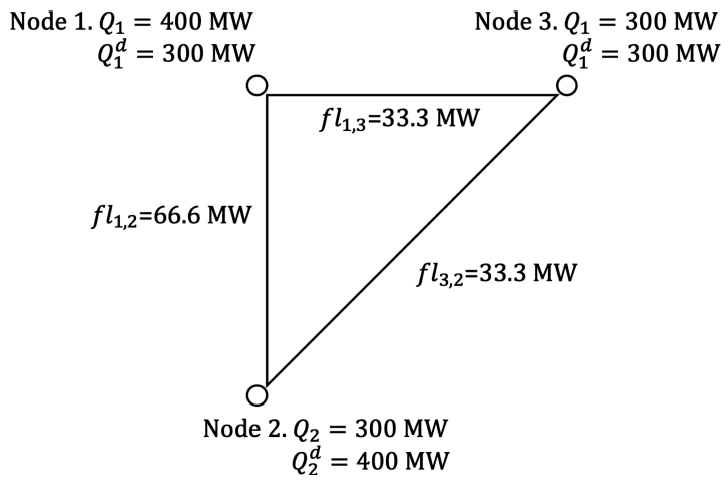
\includegraphics[scale=.4]{figure/mult_nos.png}
    \caption{Exemplo com 3 Nós - Específico}
    \label{fig:3_nodes}
\end{figure}
Teremos que a resistência do trecho $f_{1,3,2}$ é o dobro do trecho $f_{1,2}$ em virtude das distâncias. Mais ainda, sabemos que o nó 1 exporta 100 MW para o nó 2. As Leis de Kirkokff implicam:
\begin{align*}
    \begin{cases}
        f_{1,2}+f_{1,3,2}=100\\
        f_{1,2} = 2f_{1,3,2}
    \end{cases} \Rightarrow (f_{1,2},f_{1,3,2})\approx(66.6,33.3)
\end{align*}
Ora, a existência de equilíbrio depende das restrições de capacidade de transmissão. Suponha que a restrição de capacidade só possa ser ativa em $f_{1,2}$. O problema de maximização de bem-estar (simplificado) pode ser escrito como:
\begin{align*}
    \max_{q_1,q^d}&\quad U(q^d)-c_1(q_1)\\
    \text{s.a.}&\quad q_i=q^d\\
    &\quad 0\leq q_i\leq q_i^{max}\\
    &\quad f_{1,2}\le k^{max} \\
    &\quad f_{1,2}+f_{1,3,2}=100\\
    &\quad f_{1,2} = 2f_{1,3,2}
\end{align*}
Podemos simplificar as últimas 3 restrições para $\frac{2}{3}q_1\le k^{max}$. Escrevendo o Lagrangiano tal qual usual, teremos CPO:
\begin{align*}
    \frac{\partial\mathcal{L}}{\partial q_i} &= c_1 +\mu +\frac{2}{3}\chi -\lambda_1+\lambda_2 = 0 \Rightarrow -\mu = c_1+\frac{2}{3}\chi-\lambda_1 + \lambda_2
\end{align*}
Ou seja, o preço nodal é reduzido. Mais ainda, se $k^{max}=50$, naturalmente, será impossível chegar ao equilíbrio maximizador de bem-estar.

\subsection{Caso Geral}
De forma mais geral, o exemplo acima pode ser definido tal qual indicado na Figura~\ref{fig:3_nodes_gen}. Repare que o problema em questão pode ser escrito como (supondo solução interior):

\begin{figure}
    \centering
    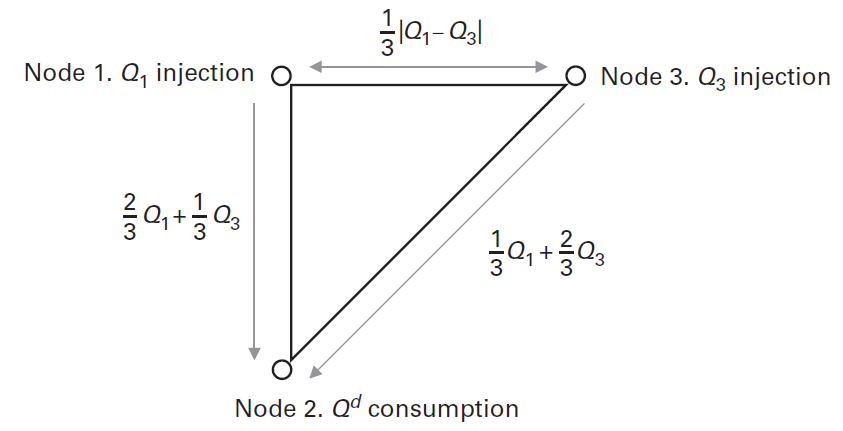
\includegraphics[scale=.4]{figure/3nos.png}
    \caption{Exemplo com 3 Nós - Geral}
    \label{fig:3_nodes_gen}
\end{figure}

\begin{align*}
    \max_{q^d,q_1,q_3}&\quad U(q^d)-c_1q_1-c_3q_3\\
    \text{s.a.}&\quad q^d=q_1+q_3\\
    &\quad\frac{1}{3}|q_1-q_3|\le k^{max}
\end{align*}
Sem perda de generalidade, suponha $q_1\ge q_3$. Teremos um Lagrangiano que implica as seguintes CPOs:
\begin{align*}
    \frac{\partial\mathcal{L}}{\partial q_1} &= 0 \Longrightarrow -\mu = c_1+\frac{1}{3}\chi\\
    \frac{\partial\mathcal{L}}{\partial q_3} &= 0 \Longrightarrow -\mu = c_3-\frac{1}{3}\chi\\ 
    \frac{\partial\mathcal{L}}{\partial q^d} &= 0 \Longrightarrow -\mu =U'(q^d)
\end{align*}
De forma que os preços nodais derivados do equilíbrio descentralizado seriam:
\begin{align*}
    p_1&: p_1\equiv c_1 = p_2 - \frac{\chi}{3}\\
    p_2&: p_2\equiv \lambda = U'(q^d)  \\
    p_3&: p_3\equiv c_3 = p_2 + \frac{\chi}{3}
\end{align*}
Novamente, na ausência de congestionamento os preços serão iguais entre todos os nós e idênticos à utilidade marginal do consumo de eletricidade. Na presença de congestionamento, produção será incentivada no terceiro nó, o mais custoso, mas permite mais geração na usina 1 (mais eficiente) por gerar contrafluxo de eletricidade - aliviando, portanto, o congestionamento da rede. Outra forma de constatar essa externalidade positiva de produção na rede é reparar que, das CPOs:
\begin{align*}
    c_3-c_1=\frac{2}{3}\chi \Longleftrightarrow \chi=\frac{3}{2}(c_3-c_2)
\end{align*}
Isto é, o valor do sistema de distribuição é maior que o diferencial dos custos marginais de produção ou, posto de outra forma, o sistema de distribuição adiciona produtividade na malha. 

Repare, também, que o segundo nó pode estar produzindo eletricidade, entretanto, sua demanda é maior que a oferta e, portanto, precisa importar do resto da rede. O raciocínio para os demais nós vale de forma simétrica. Vamos elaborar sobre essa interpretação na próxima seção.

\section{Expansão de Capacidade}
Suponha um exemplo em que existam dois nós (ou zonas), apenas, com custos marginais diferentes. O exemplo sobre o qual este se baseia está melhor explicitado no Capítulo 14.22 de \textcite{cretì_fontini_2019}. 

Suponha que exista carga e geração em ambas zonas, entretanto, que o custo marginal de produção na zona 1 seja menor que na zona 2. O problema aqui discutido pode ser graficamente representado pela Figura~\ref{fig:zones_1}. 

\begin{figure}
    \centering
    \begin{subfigure}{.45\linewidth}
        \centering
        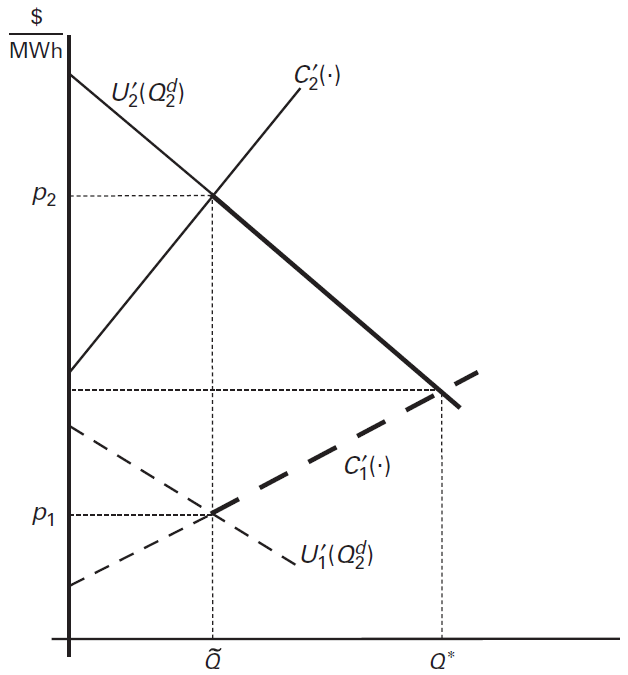
\includegraphics[scale=.3]{figure/zones_1.png}
        \caption{Sem restrições de transmissão}
        \label{fig:zones_1}
    \end{subfigure}
    \begin{subfigure}{.45\linewidth}
        \centering
        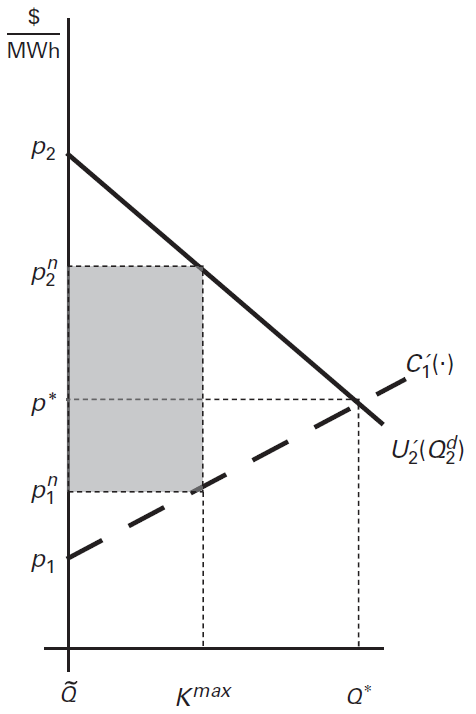
\includegraphics[scale=.3]{figure/zones_2.png}
        \caption{Com restrições de transmissão}
        \label{fig:zones_2}
    \end{subfigure}
    \caption{Problema com Duas Zonas}
\end{figure}

Note que a zona 1, por ser mais eficiente, possibilita a existência de uma demanda adicional na zona 2 que não seria possível caso elas não estivessem conectadas. Desta forma, a zona 1 se torna uma exportadora de energia, enquanto a zona 2 uma importadora.

Suponha, agora, que exista uma restrição de transmissão denotada por $k^{max}$. Note que o problema na zona 2 muda e torna-se tal qual descrito na Figura~\ref{fig:zones_2}. Seja a área sombreada a remuneração do operador pelo uso do sistema de distribuição, de forma similar à seção anterior, denotada por CR (\textit{congestion rent}). 

O bem-estar decorrente \textbf{do fluxo} de energia entre as zonas, considerando a remuneração do operador, pode ser escrito como:
\begin{align*}
    W&= \underbrace{(p_2^n-p_1^n)k^{max}}_{CR}+\underbrace{\frac{1}{2}(p_1^n-p_1)k^{max}}_{PS}+\underbrace{\frac{1}{2}(p_2+p_2^n)k^{max}}_{CS}\\
    &=\frac{(p_2^n-p_1^n)+(p_2-p_1)}{2}k^{max}
\end{align*}
onde PS denota o excedente do produtor (\textit{productor surplus}) e CS o excedente do consumidor (\textit{consumer surplus}).

\subsection{Análise de Bem-Estar}
Note que a existência de congestionamento implica consumo de eletricidade abaixo do ótimo ($k^{max}<q^*$). O próximo passo natural ao economista é mensurar essa perda de bem-estar, chamado de "peso-morto" (\textit{deadweight loss}). Graficamente, ela pode ser compreendida como o triângulo formado entre $k^{max}$ e $q^*$ na Figura~\ref{fig:zones_2}. Analiticamente, definimos:
\[\textit{DWL}(k^{max}) = \frac{1}{2}\Big[\Big(p_2^n(k^{max})-p_1^n(k^{max})\Big)\Big(q^*-q_1(k^{max})\Big)\Big]\]
onde explicitamos as variáveis que são função de $k^{max}$ e $q_1(k^{max})$ é a quantidade exportada da zona 1 para a 2 dado o nível $k^{max}$ de capacidade de transmissão. 

Ora, então o \textbf{operador maximizador de bem-estar} visa minimizar o \textit{DWL}. Esse problema pode ser escrito como:
\begin{align*}
    \min_{k^{max}}\quad \textit{DWL}(k^{max})
\end{align*}
Implicando CPO:
\begin{align*}
    \frac{\partial\textit{DWL}}{\partial k^{max}} = 0 &\Longleftrightarrow \frac{1}{2}\Big[(p_2^{n'}-p_1^{n'})(q^*-q_1)-(p_2^n-p_1^n)q_{1}' \Big]\\
    &\Longleftrightarrow (p_2^n-p_1^n)q_{1}' = (p_2^{n'}-p_1^{n'})(q^*-q_1)
\end{align*}
Sabemos que quando há congestionamento $q_1(k^{max})=q_1=k^{max}$, implicando $q_1'=1$. Portanto, a equação acima simplifica para
\[p_2^n-p_1^n = (p_2^{n'}-p_1^{n'})(q^*-k^{max})\]
Seja $k^{max^*}$ t.q. $k^{max^*}=q^*$, implicando $p_1^n=p_2^n=p^*$. Repare que esse $k^{max^*}$ atende à equação acima. Mais ainda, pelo teorema do valor médio, só existe uma raiz para o polinômio característico da função em questão i.e. só há um valor $k^{max^*}$ que iguala o lado esquerdo ao direito.

Ora, então podemos afirmar que, no ótimo, o operador irá aumentar a capacidade de forma a não haver nenhum peso-morto no sistema, ainda que às custas de sua remuneração - que será 0 no ótimo.

Isso nos indica que, na solução descentralizada, o equilíbrio encontrado será diferente. Analiticamente, observe que o \textbf{problema do operador maximizador de lucro} é dado por:
\begin{align*}
    \max_{k^{max}}\quad \Big(p_2^n(k^{max})-p_1^n(k^{max})\Big)k^{max}
\end{align*}
Implicando CPO:
\[p_2^n-p_1^n=-(p_2^{n'}-p_1^{n'})k^{max}\]
Novamente, pelo teorema do valor intermediário, só existe um $k^{max,SO}$ que resolve a equação acima. Lembre que quando $k^{max}=k^{max^*}$, temos $p_2^n-p_1^n=0\neq -(p_2^{n'}-p_1^{n'})k^{max}$. Portanto, deve ser que $k^{max,SO}<k^{max^*}$.

Isto é, concluímos que no equilíbrio descentralizado haverá menos capacidade que no ótimo - resultado típico de problemas com externalidades positivas.

\subsection{Custos de Expansão}
Suponha, agora, que realizar a expansão seja custoso. Podemos reescrever o \textbf{problema centralizado} como:
\begin{align*}
    \min_{k^{max}}\quad \textit{DWL}(k^{max}) + \underbrace{\beta k^{max}}_{\text{custo da expansão}}
\end{align*}
Implicando CPO:
\[p_2^n-p_1^n = (p_2^{n'}-p_1^{n'})(q^*-k^{max})+2\beta\]
Novamente, só existe um valor $k^{max,\beta}$ que resolve a equação acima. Mais ainda, visto que $\beta>0$, temos que  $k^{max,\beta}<k^{max^*}$ (argumento similar ao da subseção anterior). Portanto, caso existam custos de expansão do sistema de distribuição, haverá \textit{DWL} no ótimo. Repare que podemos reescrever a equação acima como:
\[\frac{1}{2}\Big[p_2^n-p_1^n - (p_2^{n'}-p_1^{n'})(q^*-k^{max})\Big]=\beta\]
Ou seja, o nível ótimo de capacidade será aquele que faz com que o benefício marginal da expansão do sistema de distribuição se iguale ao custo marginal de expandí-lo.

De forma análoga, teremos que o \textbf{problema descentralizado} implica a seguinte CPO:
\[p_2^n-p_1^n+(p_2^{n'}-p_1^{n'})k^{max}=\beta\]
Argumento similar segue, de forma a demonstrar que $k^{max,SO,\beta}$, solução da equação acima, é tal que $k^{max,SO,\beta}<k^{max,SO}<k^{max^*}$. Entretanto, note que nada pode ser dito quando à $k^{max,\beta}$ i.e. $k^{max,SO,\beta}\gtrless k^{max,\beta}$. Ou seja, na presença de custos de expansão, é possível que a solução descentralizada esteja mais próximo do ótimo do que no caso sem custos de expansão. 
\chapter{Aquecimento Global e Eletricidade}
\localtableofcontents 

Este capítulo é baseado nas notas de aula do curso, ministrado em 17/08/2023, e no capítulo 24 de \textcite{cretì_fontini_2019}.

\section{Preço de Carbono e Mercados de Eletricidade}
Uma das formas que os economistas encontraram para ajudar a mitigar o problema do aquecimento global é precificar o carbono emitido na produção dos bens - inclusive eletricidade. Essa prática é intuitiva do ponto de vista econômico, pois a emissão de gases poluentes configura uma externalidade negativa - e a teoria microeconômica diz que existe um preço ótimo da externalidade tal que faça o problema descentralizado convergir para o problema do planejador central.

Na prática, existem algumas formas de se construir esse mercado de carbono. Uma delas é dar às empresas licenças para emissões proporcionalmente às suas emissões históricas, por exemplo, e permitir que elas comercializem com as demais por mais licenças a fim de expandir as emissões. Independente do sistema de como se dão as licenças, o processo de distribuí-las gratuitamente é chamado de "\textbf{apadrinhamento}" (em contraponto à um leilão, por exemplo).

Nesse sistema, o lucro das firmas irá subir sempre, pois elas conseguem reverter 100\% do aumento de custos para o consumidor. Isso se dá pois o custo marginal de produção se mantém constante, mas o custo-oportunidade de geração aumenta, pois as firmas podem vender as licenças no mercado. Graficamente, haverá um deslocamento da curva de oferta para a esquerda, tal qual exemplificado na Figura~\ref{fig:gdfth}.

\begin{figure}
    \centering
    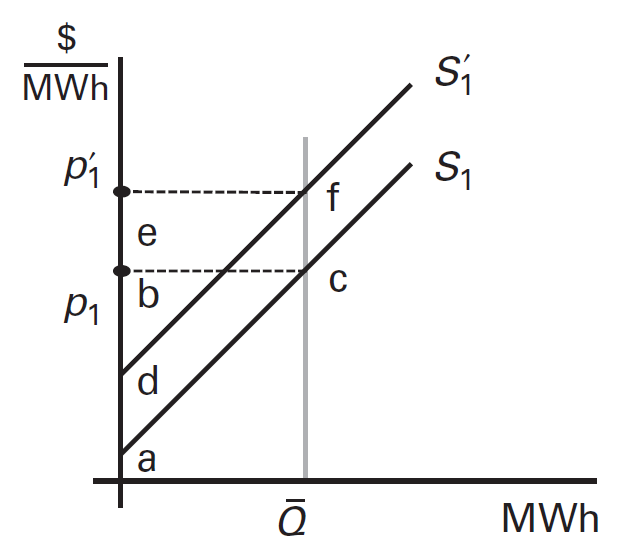
\includegraphics[scale=.25]{figure/grandfather.png}
    \caption{Consequências do Apadrinhamento}
    \label{fig:gdfth}
\end{figure}

Entretanto, caso as licenças tivessem sido vendidas em um leilão, obtê-las muda diretamente o custo marginal das firmas - podendo ou não, portanto, alterar a ordem de mérito. Caso não haja nenhuma mudança na ordem de mérito, as conclusões serão as mesmas do caso de apadrinhamento i.e. haverá \textit{pass-through} completo para o consumidor. Caso a ordem mude, contudo, então haverá \textit{pass-through} parcial, apenas. Isso pode ser visto graficamente na Figura~\ref{fig:cc}, onde a existência das licenças faz com que o aumento do preço marginal do sistema seja menor que o aumento no custo marginal da firma marginal - i.e. não há \textit{pass-through} completo.

\begin{figure}
    \centering
    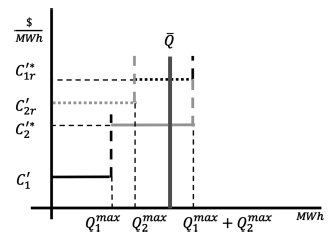
\includegraphics[scale=.6]{figure/cc_meritorder.png}
    \caption{Mudança na Ordem de Mérito}
    \label{fig:cc}
\end{figure}

%\part{Physics}
%\input{./chapter/quantum_mechanics.tex}
% \input{./chapter/quantum_field_theory.tex}

%\begin{appendices}
%\input{./chapter/appendix_formula.tex}
%\end{appendices}

\backmatter

%%%%%%%%%%%%%%% Reference %%%%%%%%%%%%%%%

\printbibliography[heading=bibintoc]
\printindex

\end{document}

